% Compile with: lualatex -shell-escape <file>.tex
\documentclass[a4paper]{article}
\usepackage{htl-template}
\begin{document}
\bibliographystyle{IEEEtran}
\pagestyle{htl}
\pagenumbering{roman}
\section*{\topic}
\par\noindent\rule{\textwidth}{0.4pt}

Laboratory protocol
Excercise \exerciseNumber: \topic

\begin{figure}[h]
	
\includegraphics[scale=0.4]{images/miniheraDogDoorbell.png}
	\centering
\end{figure}

\vspace*{\fill}
Subject:	\subject

Class:	\className

Name:	\studentone, \studentwo

Gruppenname/Nummer: \groupname /\groupnumber

Supervisor: 	\teacher \teachertwo

Exercise dates:	 16.05.2025 | 06.06.2025

Submission date: 10.06.2025


\newpage
\tableofcontents
\newpage
\pagenumbering{arabic}

\section{Task definition}
This task focuses on the setup and subsequent attack of a WLAN network. The initial phase, "Übung 10: Einrichten eines WLAN-Netzwerks," guides students through provisioning a WLAN. This involves configuring an Access Point (AP), planning channel usage, setting up Network Address Translation (NAT) and a DHCP service, and ensuring full connectivity between wireless and wired clients. Students configure a router with NAT, establish a DHCP server, and set up the AP with \texttt{WPA2} security, assessing password strength and measuring channel utilization. Connectivity tests confirm communication within the network and to the internet. Access Point Isolation is also explored, with a bonus task involving its configuration and demonstration of its effects. \nl
The second phase, "Übung 11: Angriff eines WLAN-Netzwerks," delves into ethical hacking using the \texttt{aircrack-ng} framework. This begins with checking WLAN card recognition and enabling monitoring mode using tools like \texttt{iw dev}, \texttt{iwconfig}, and \texttt{wifite}, followed by \texttt{airmon-ng start <WLAN-Interface>}. Students then use \texttt{airodump-ng <WLAN-Interface>} to monitor WLANs and identify network details such as BSSID and channel. A deauthentication attack is performed using \texttt{aireplay-ng --deauth <Anzahl der Pakete> -a <BSSID> -D <WLAN-Interface>}, analyzing its impact on connected clients. Finally, the task culminates in cracking the WLAN password using \texttt{airodump-ng} to capture the WLAN handshake (saved as a \texttt{.pcap} file), viewing it in \texttt{Wireshark}, and then employing \texttt{aircrack-ng -w password.lst -b <BSSID> <CaptureFile>.pcap} with a password list. A bonus challenge involves using \texttt{Hashcat} for password cracking, requiring \texttt{hcxpcapngtool -o <Datei-name>.22000 -E essid <CaptureFile>.pcap} for file conversion and leveraging potentially more powerful computational resources.\footnote{This summary of the task definition was created using Gemini 2.5 Flash using the Task definition as context.}
\section{Summary}
In this exercise, a WLAN network was established and subsequently attacked. The setup phase involved configuring a router for NAT and DHCP, enabling the internal network to access the internet and clients to receive IP addresses from the \(172.28.0.0/24\) subnet. The router was configured with an access list for NAT and an \texttt{ip nat inside source} command for overload PAT, ensuring multiple internal hosts could share a single public IP. DHCP was configured with a pool for the \(172.28.0.0/24\) network, specifically excluding the router's, a static server's, and the access point's IP addresses. The router's internet connectivity and DHCP assignments were thoroughly verified through ping tests and IP address checks on connected devices.\nl
The Access Point was reset and configured via its web interface with a static IP address within the defined internal subnet. A Wi-Fi network named \texttt{3AHITN-GRP-12} was created on the \(2.4\) GHz radio, initially with isolation disabled to allow client-to-client communication. Security was set to \texttt{WPA2} with the password \texttt{Passwort2025!}. The strengths of various security algorithms (\texttt{WEP}, \texttt{WPA}, \texttt{WPA2-Personal}, \texttt{WPA2-Enterprise}) and the chosen password were assessed. Channel usage was carefully monitored using \texttt{NetSpot} to inform channel selection and avoid conflicts with existing networks. Connectivity was then confirmed by pinging between wireless clients, between wireless and wired clients, and from a wireless client to the internet. The concept of Access Point Isolation was explained and demonstrated, showing how it prevents communication between wireless clients, yet notably does not hinder packet sniffing.\nl
The attack phase commenced with setting up a \texttt{Wi-Fi} adapter for monitoring mode. This involved installing necessary drivers for a \texttt{RTL8821AU} chipset and activating monitor mode using commands like \texttt{iw dev} or the \texttt{wifite} utility. The \texttt{airmon-ng} tool was then used to enable monitor mode and manage any conflicting processes. Subsequently, \texttt{airodump-ng} was employed to scan for \texttt{Wi-Fi} networks, gather critical information such as the BSSID and channel for the target network \texttt{3AHITN-GRP-12}, and capture raw \(802.11\) frames from the target access point and its associated clients. A deauthentication attack was performed with \texttt{aireplay-ng} to disconnect a specific client and force a \texttt{WPA2} 4-Way Handshake, which was successfully captured and verified.\nl
The captured 4-Way Handshake was then analyzed in \texttt{Wireshark} (or \texttt{Termshark}) using the \texttt{eapol \&\& !eap} filter to isolate the relevant frames. Each of the four \texttt{EAPOL} (Extensible Authentication Protocol over LANs) frames was dissected, with detailed explanations of key fields including Descriptor Type, Key Information, Key Length, Key Replay Counter, Key Nonce, Key RSC, Key MIC, Key Data Length, and Key Data. Visual representations of each handshake message were provided, illustrating the exchange of ANonce, SNonce, MICs, and GTK. Finally, the captured handshake was used with \texttt{aircrack-ng} and a wordlist to crack the \texttt{Wi-Fi} password. A bonus task involved attempting to crack a personal \texttt{Wi-Fi} password using \texttt{hcxpcapngtool} for capture conversion and \texttt{Hashcat} for a brute-force attack, demonstrating the significant difficulty of cracking long, complex passwords. \footnote{This summary of the exercise was created using Gemini 2.5 Flash using my tex file as context.}
\newpage

\section{Complete network topology of the exercise}
\begin{figure}[h]
	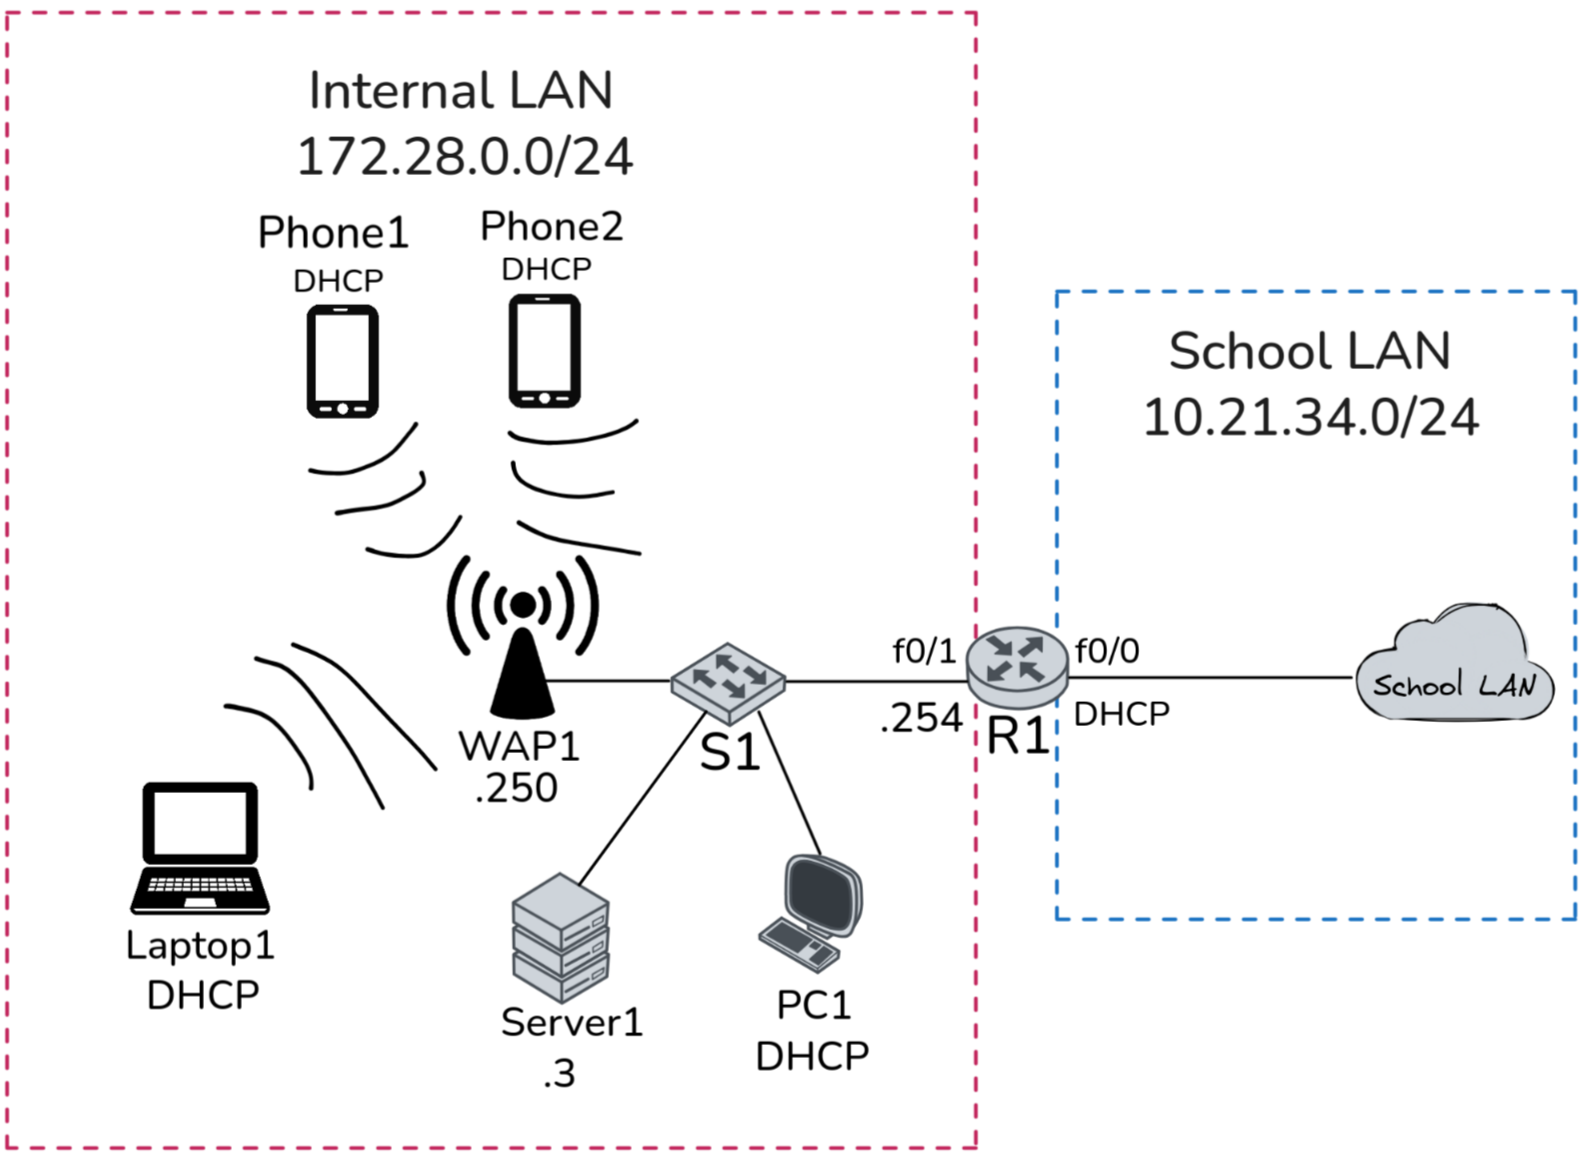
\includegraphics[scale=0.3]{images/topo.png}
	\centering
	\caption{Complete network topology}
\end{figure}

\newpage
\section{Exercise Execution}

\subsection{Setting up the Network}
To set up this exercise, we first had to build the topology from Figure 1 and configure the devices accordingly.

\subsubsection{Configuring the Router}
The router needs to have NAT configured since internet access will be required for this exercise. \nl
There are multiple approaches to creating NAT, which include Overloading or Port Address Translation (PAT), Static Port Address Translation (Port Redirection), or Static NAT.\cite{noauthor_how_nodate} \nl
Here, the most frequently used approach will be employed, which is \texttt{PAT}, where multiple connections from internal hosts are \textbf{multiplexed} into a \texttt{single} registered public IP address using different source port numbers. This allows for \texttt{65,536} translations per public IP and is used by basically every home since they typically have a single router that serves as the only gateway and has NAT to the ISP. Rarely do non-enterprise customers get their own static IP, and thus sometimes even multiple homes are NATed together into a single public IP which is called CGNAT (Carrier-Grade NAT).\cite{noauthor_how_nodate, noauthor_what_nodate-1} \nl
This approach also works inside an already NATed network, as we did here. Inside the school network, we used our router to create a NAT with the school network, giving us internet access. For this, we used the following commands.
\begin{listing}[ht]
\begin{minted}{bash}
# allowing addresses in the 172.28.0.0/24 subnet to be translated
access-list 1 permit 172.28.0.0 0.0.0.255
# using the above list of addresses to be allowed to get translated and 
# specifying the interface on which the school network comes in and 
# specifying the NAT type with the overload keyword
ip nat inside source list 1 interface f0/0 overload
# setting the port f0/0 to be the source of the school network, which in 
# this case is the "internet"
interface f0/0
ip nat outside
# setting the port for our LAN
interface f0/1
ip nat inside
\end{minted}
\caption{Router NAT configuration commands}
\end{listing} \nl
This configuration can be verified by running the command \texttt{ip address dhcp} to obtain an IP address from the school's DHCP server for our router, which can then be viewed using \texttt{show ip int br}. From the DHCP server, we also received a gateway and static routes to reach the internet, which are displayed using \texttt{show ip route}. Lastly, Google is pinged to demonstrate connectivity. All of these steps can be examined in Figure 2 on the next page. \newpage
\begin{figure}[!ht]
	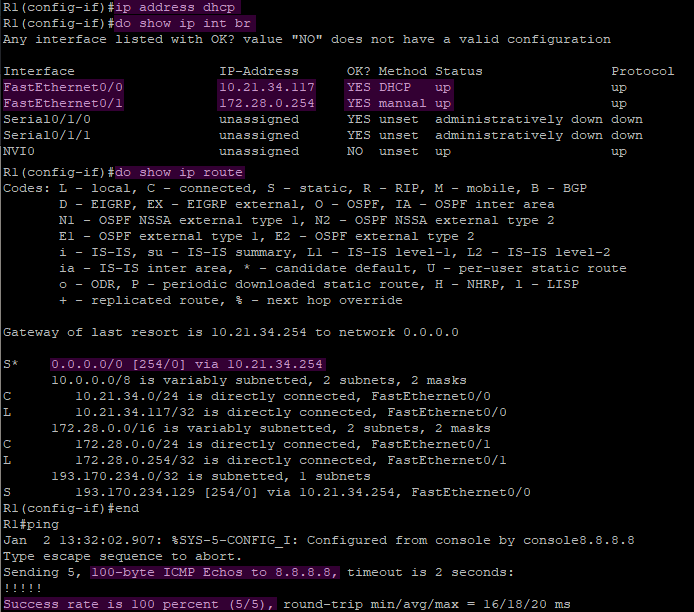
\includegraphics[scale=0.5]{images/nat.png}
	\centering
	\caption{Verifying the NAT configuration}
\end{figure}\nl
Next, DHCP needs to be configured on the router so that clients can obtain IP addresses. To do this, first, a DHCP pool has to be created using the \texttt{ip dhcp pool} command along with a desired name for the pool in global configuration mode. \nl
Then, the network from which to hand out IP addresses is specified using the \texttt{network} command along with the network address and the subnet mask. \nl
The default router and DNS server are set afterward, as well as excluding three addresses to align with the topology using the \texttt{ip dhcp excluded-address} command. The commands used are as follows:

\begin{listing}[ht]
\begin{minted}{bash}
# creating the pool
ip dhcp pool R1_Intern_LAN
# setting the network
network 172.28.0.0 255.255.255.0
# setting the default router
default-router 172.28.0.254
# using the school's DNS server
dns-server 193.170.234.183
# excluding IP addresses from the pool
ip dhcp excluded-address 172.28.0.3
ip dhcp excluded-address 172.28.0.254
ip dhcp excluded-address 172.28.0.250
\end{minted}
\caption{Router DHCP configuration commands}
\end{listing} \nl
This configuration will be verified in two sections after the access point is added and clients are on the network, testing its connectivity.
\subsubsection{Configuring the Access Point}
To configure the access point, first, we reset it by holding the reset button on the back for 15 seconds in case it has already been configured. \nl
Once it has been reset, it is plugged into the switch, which does not need to be configured and already has Power over Ethernet (PoE), so no power supply is needed to power the access point, nor is any configuration required for the switch. \nl
To access the access point's configuration, a computer is connected to the same switch, and its IP address is changed to the \texttt{192.168.1.0/24} subnet. Then, at \texttt{192.168.1.252}, its configuration can be accessed as stated in the manual on pages 7 and 8 \cite{noauthor_lapac1200_nodate}. \nl
To set the correct IP address of the access point, the configuration tab is opened, and under \texttt{LAN} \rightarrow \texttt{Network Setup}, the IP is set to static and configured to the correct address according to the topology, as can be seen in Figure 3. \nl
\begin{figure}[!ht]
    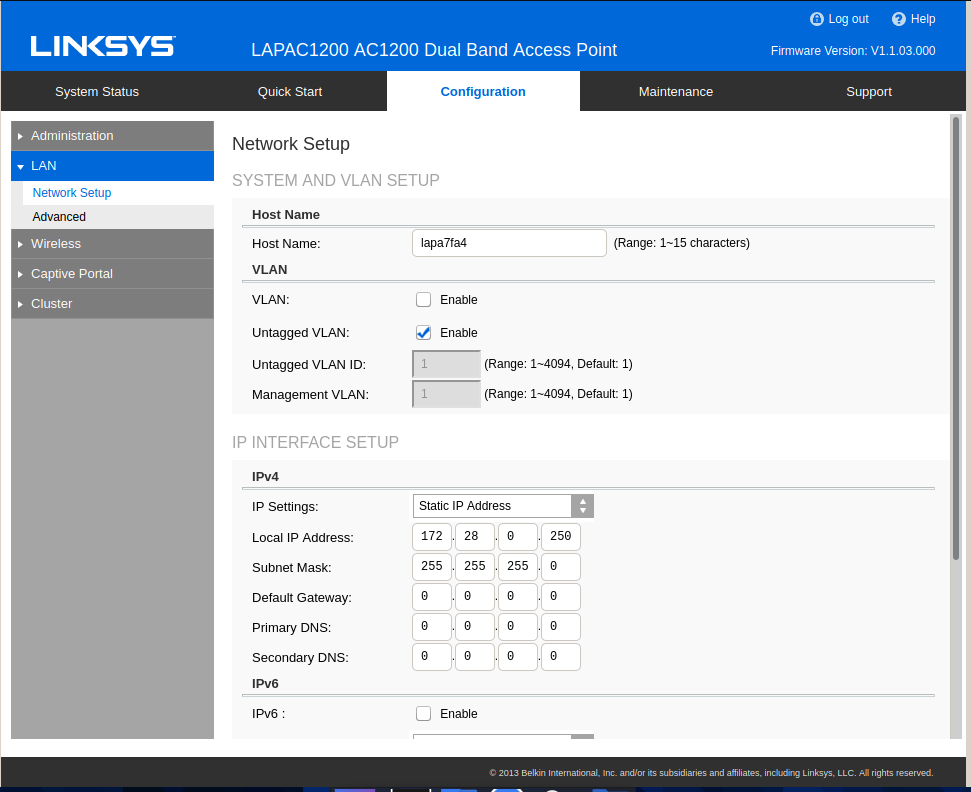
\includegraphics[scale=0.5]{images/A2.1-AP1-ip.png}
    \centering
    \caption{Changing the network settings of the access point}
\end{figure} \nl
The Wi-Fi network to set up is configured in the \texttt{Wireless} \rightarrow \texttt{Basic Settings} tab for \texttt{Radio 1}, which means configuring the \texttt{2.4 GHz} radio. Below, under \texttt{SSID}, the desired SSID is set, and importantly, the isolation checkbox is unchecked so that wireless devices are not isolated and can ping each other. In section 4.1.4, isolation will be discussed further, but for now, it remains off. Lastly, the channel is set to auto, which can be seen with the other configurations in Figure 4. On the day of the lab, the two rooms were filled with access points, and the entire \texttt{2.4 GHz} spectrum was congested, leaving no free channel to select. This can be observed in Figure 5, where \texttt{NetSpot} was used to analyze the usage of the channels. \newpage
\begin{figure}[!ht]
    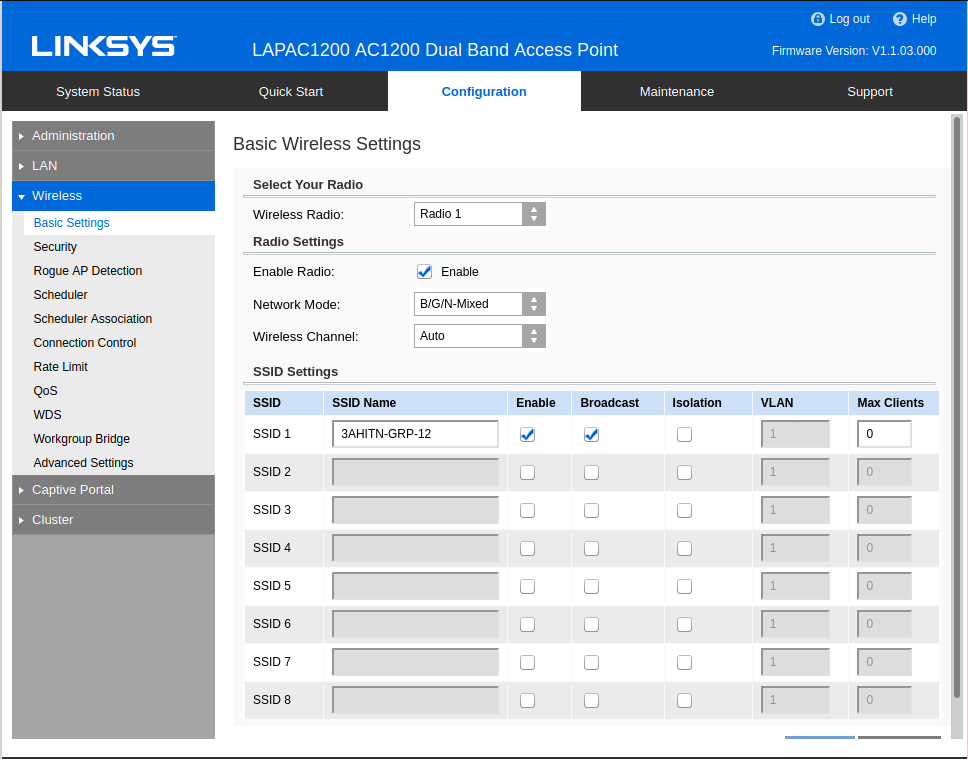
\includegraphics[scale=0.5]{images/A2.1-AP1.png}
    \centering
    \caption{Setting up the \texttt{Wi-Fi} Network}
\end{figure}
\begin{figure}[!ht]
    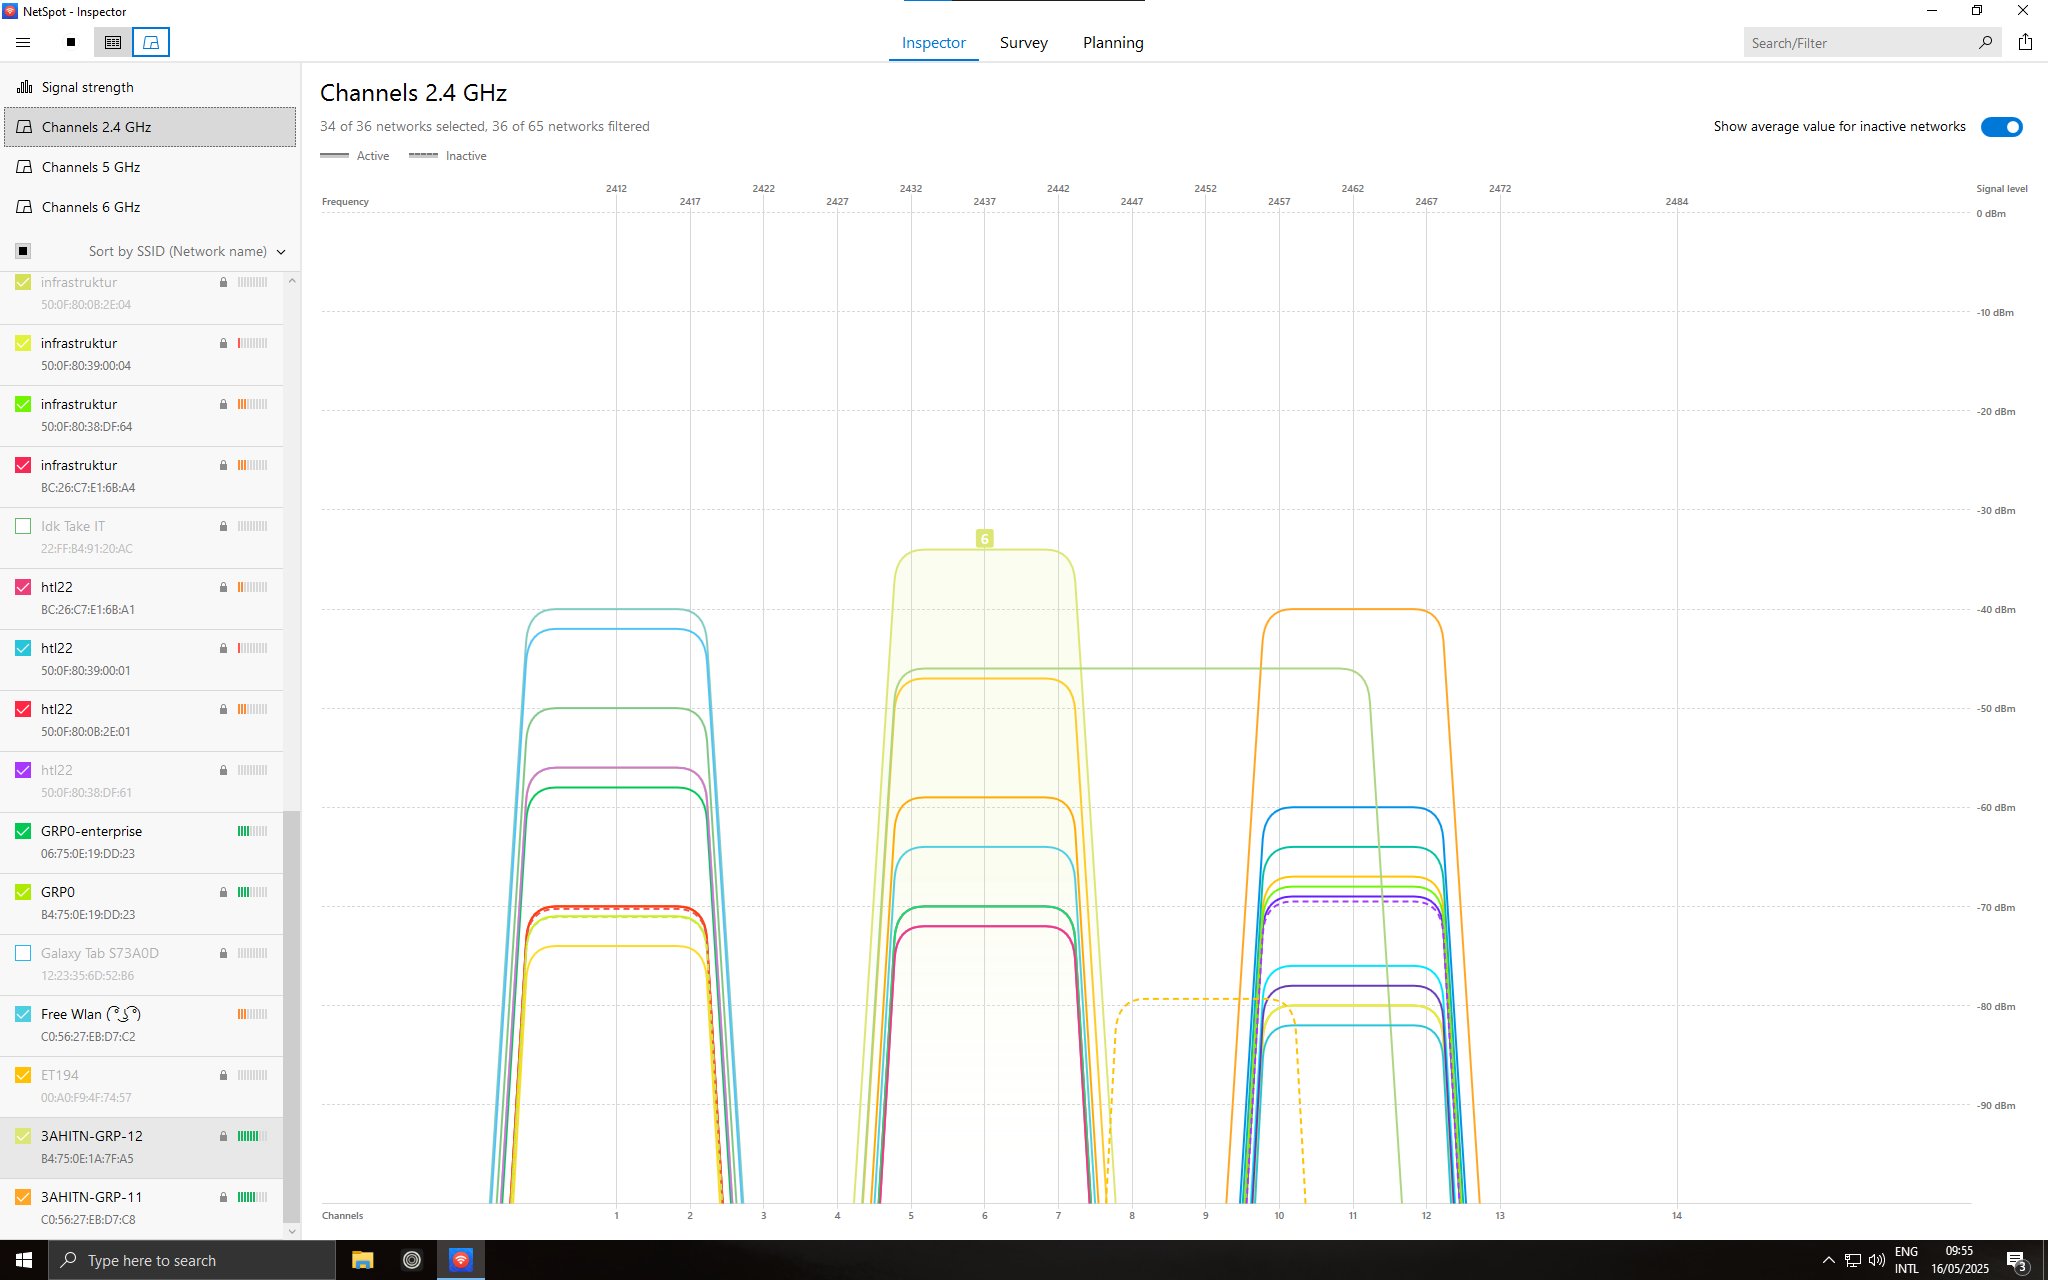
\includegraphics[scale=0.23]{images/wifichan.png}
    \centering
    \caption{Viewing the usage of the channels in the \texttt{2.4 GHz} spectrum}
\end{figure} \newpage\nl
Now, under the \texttt{Wireless} \rightarrow \texttt{Security} tab, the \texttt{SSID} is selected for configuration, which in our case is the previously created \texttt{SSID}. The Password/Pre-Shared Key to use is \texttt{Passwort2025!}, as specified in the task definition, and \texttt{WPA2} is selected as the encryption algorithm, which can be seen in Figure 6. \nl
As stated in the access point's manual on pages 32 to 43, it offers \texttt{WEP, WPA2-Personal, WPA/WPA2-Personal, WPA2-Enterprise, WPA/WPA2-Enterprise}, and \texttt{RADIUS}. The only two relevant options are \texttt{WPA2-Personal} and \texttt{WPA2-Enterprise}, since the other options that use \texttt{WPA} or \texttt{WEP} are obsolete and can be easily compromised with minimal computational efford. The most secure of the relevant options is \texttt{WPA2-Enterprise}, as the pairwise master key is regenerated for each session compared to \texttt{WPA2-Personal} \cite{noauthor_wpa2_nodate, noauthor_lapac1200_nodate}. \nl
The password \texttt{Passwort2025!} is also not very secure, as an attacker could use a wordlist and automatically generate variants of it. This could be cracked quickly by adding human-like variants, such as appending the current year and a random special character, and then repeating this for every entry in the wordlist. Bitwarden's password test tool estimates that this password would be cracked in 18 hours, as seen in Figure 7. \nl
\begin{figure}[!ht]
    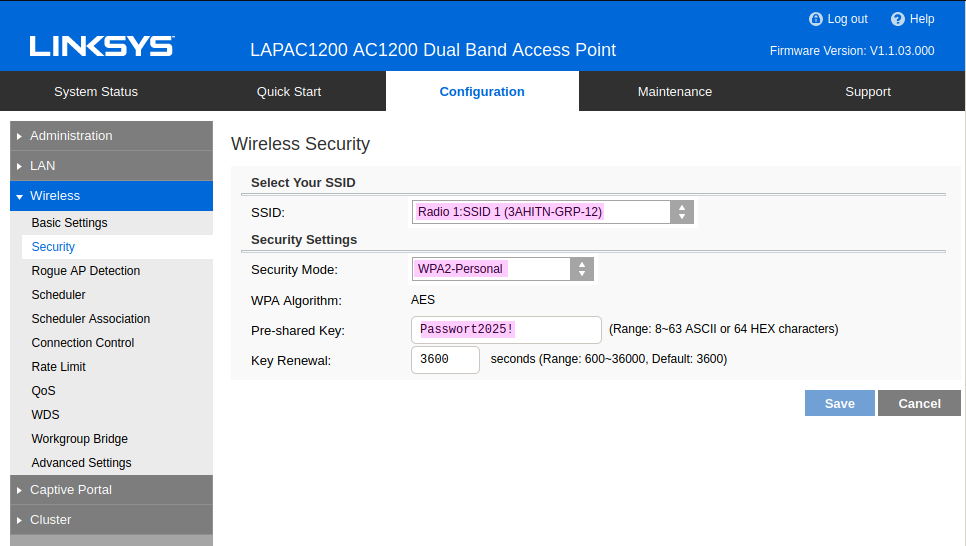
\includegraphics[scale=0.48]{images/A2.1-AP1-wpa.png}
    \centering
    \caption{Setting up the Security settings for the \texttt{Wi-Fi} Network}
\end{figure}
\begin{figure}[!ht]
    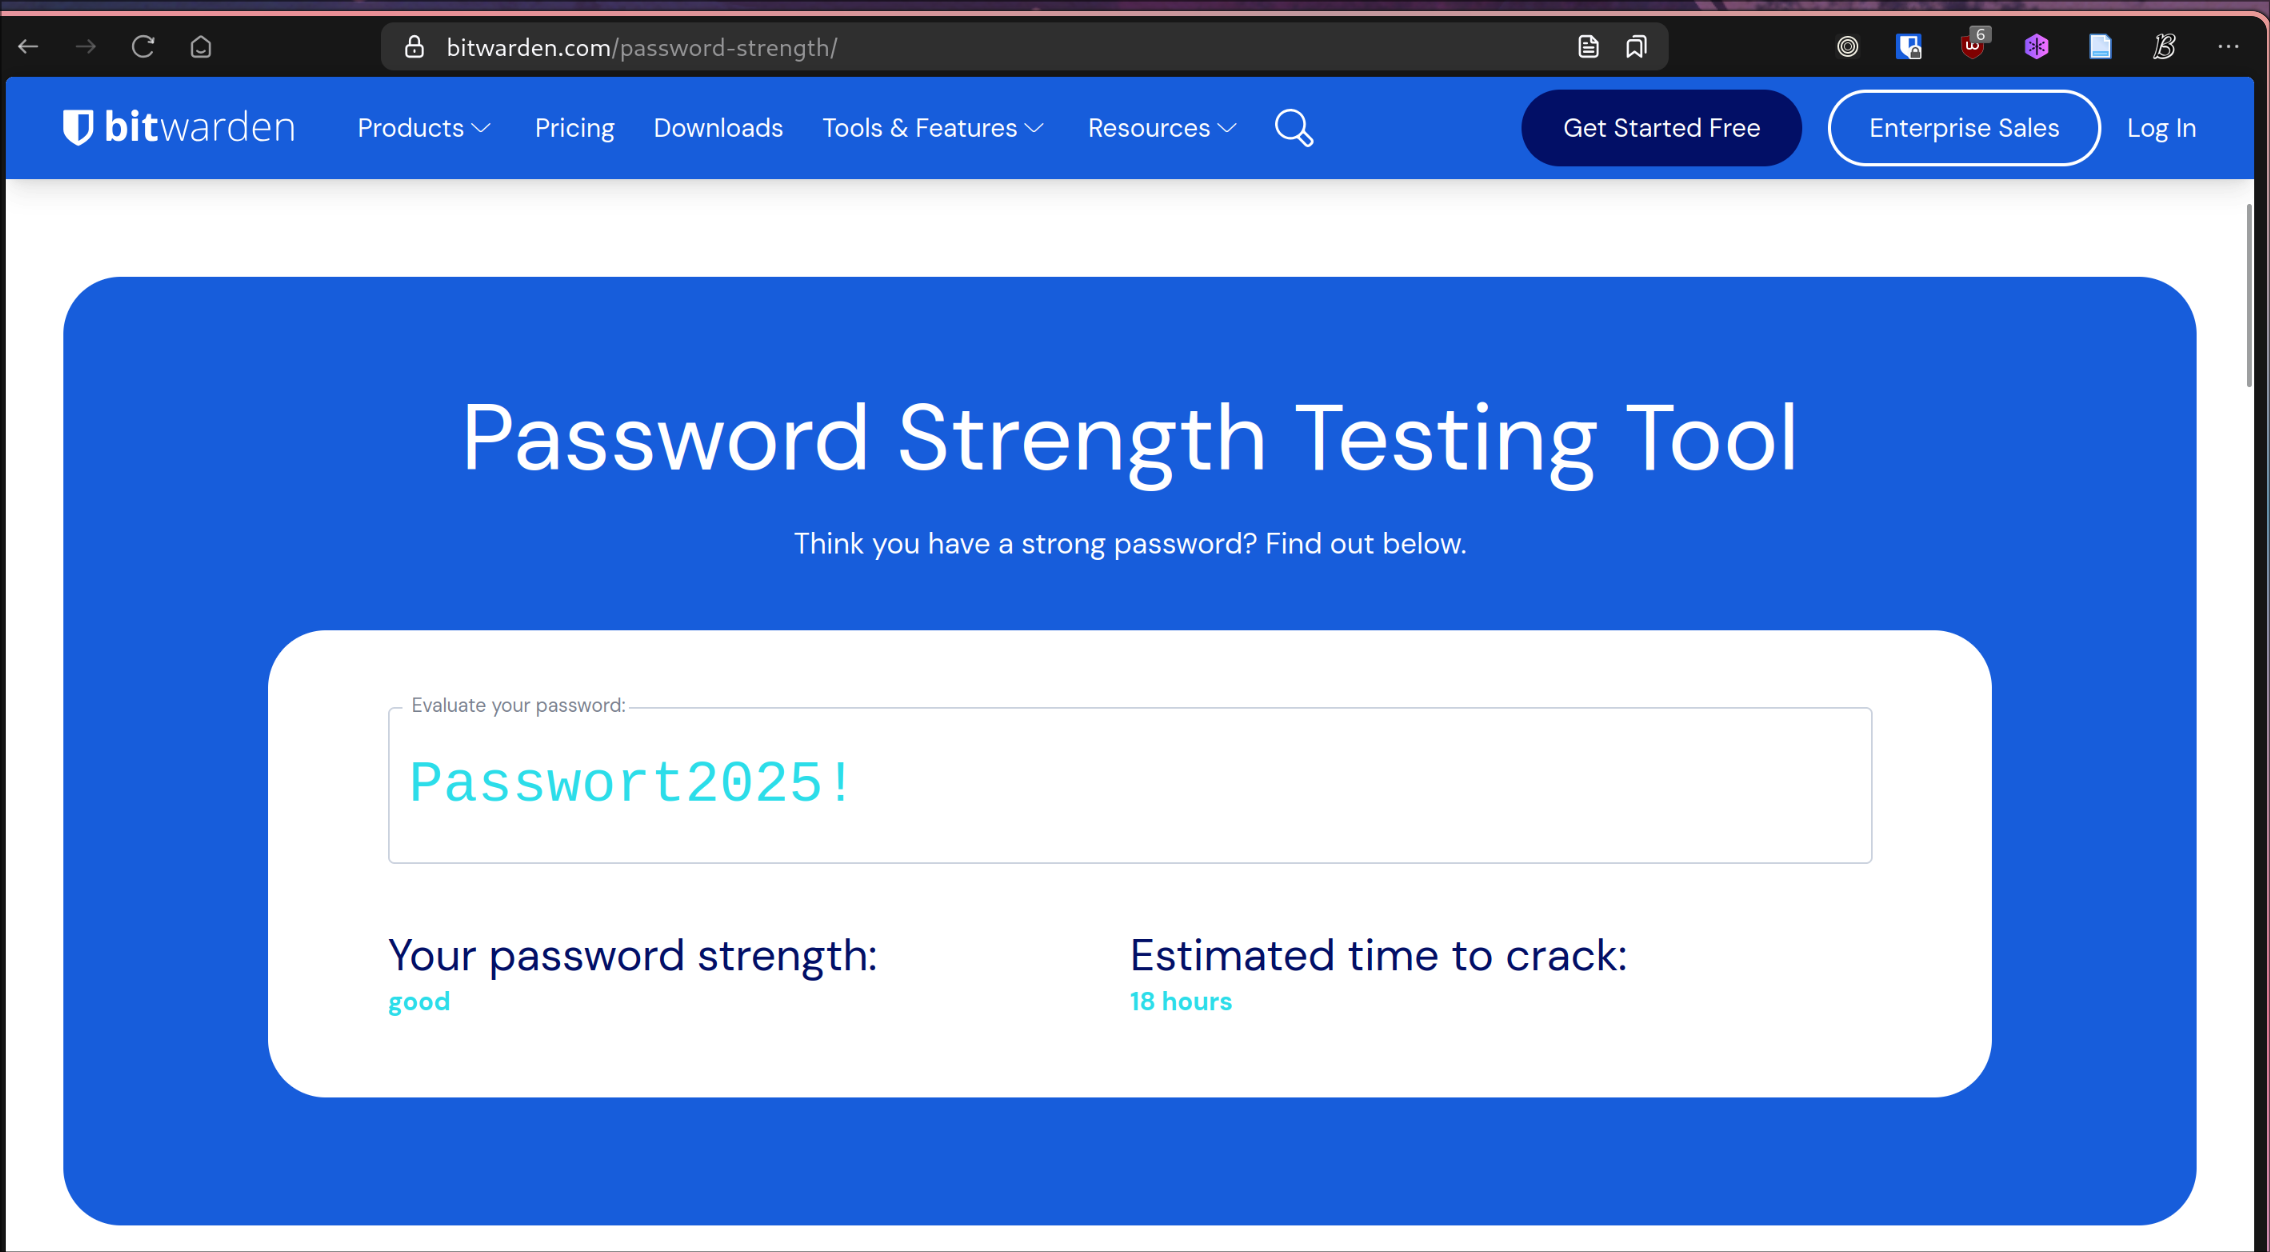
\includegraphics[scale=0.15]{images/pwthingtest.png}
    \centering
    \caption{Testing the password's strengh}
\end{figure} \newpage
\subsubsection{Testing connectivity and DHCP addreses}
To verify the DHCP assignments and the connectivity, the IP of the attacker's laptop, which at the time was plugged in instead of using the wireless network, received the \texttt{.1} address assigned, as shown in Figure 8. This figure also displays two phones as wireless clients and their assigned IPs. Figure 9 shows one of the phones pinging the other phone, the laptop, and Google to verify the connectivity of a wireless device to a wired one, between two wireless devices, and from a wireless device to the internet. To ping with the phone, the \texttt{ping} command was used inside the \texttt{Termux} mobile app, which is available on the Google Play Store or on F-Droid for Android phones. \footnote{Figure 9 consists of multiple screenshots manipulated together using Photopea to save space in the document, eliminating the need for multiple figures and allowing everything to fit cleanly on a single page. :3}
\begin{figure}[!ht]
    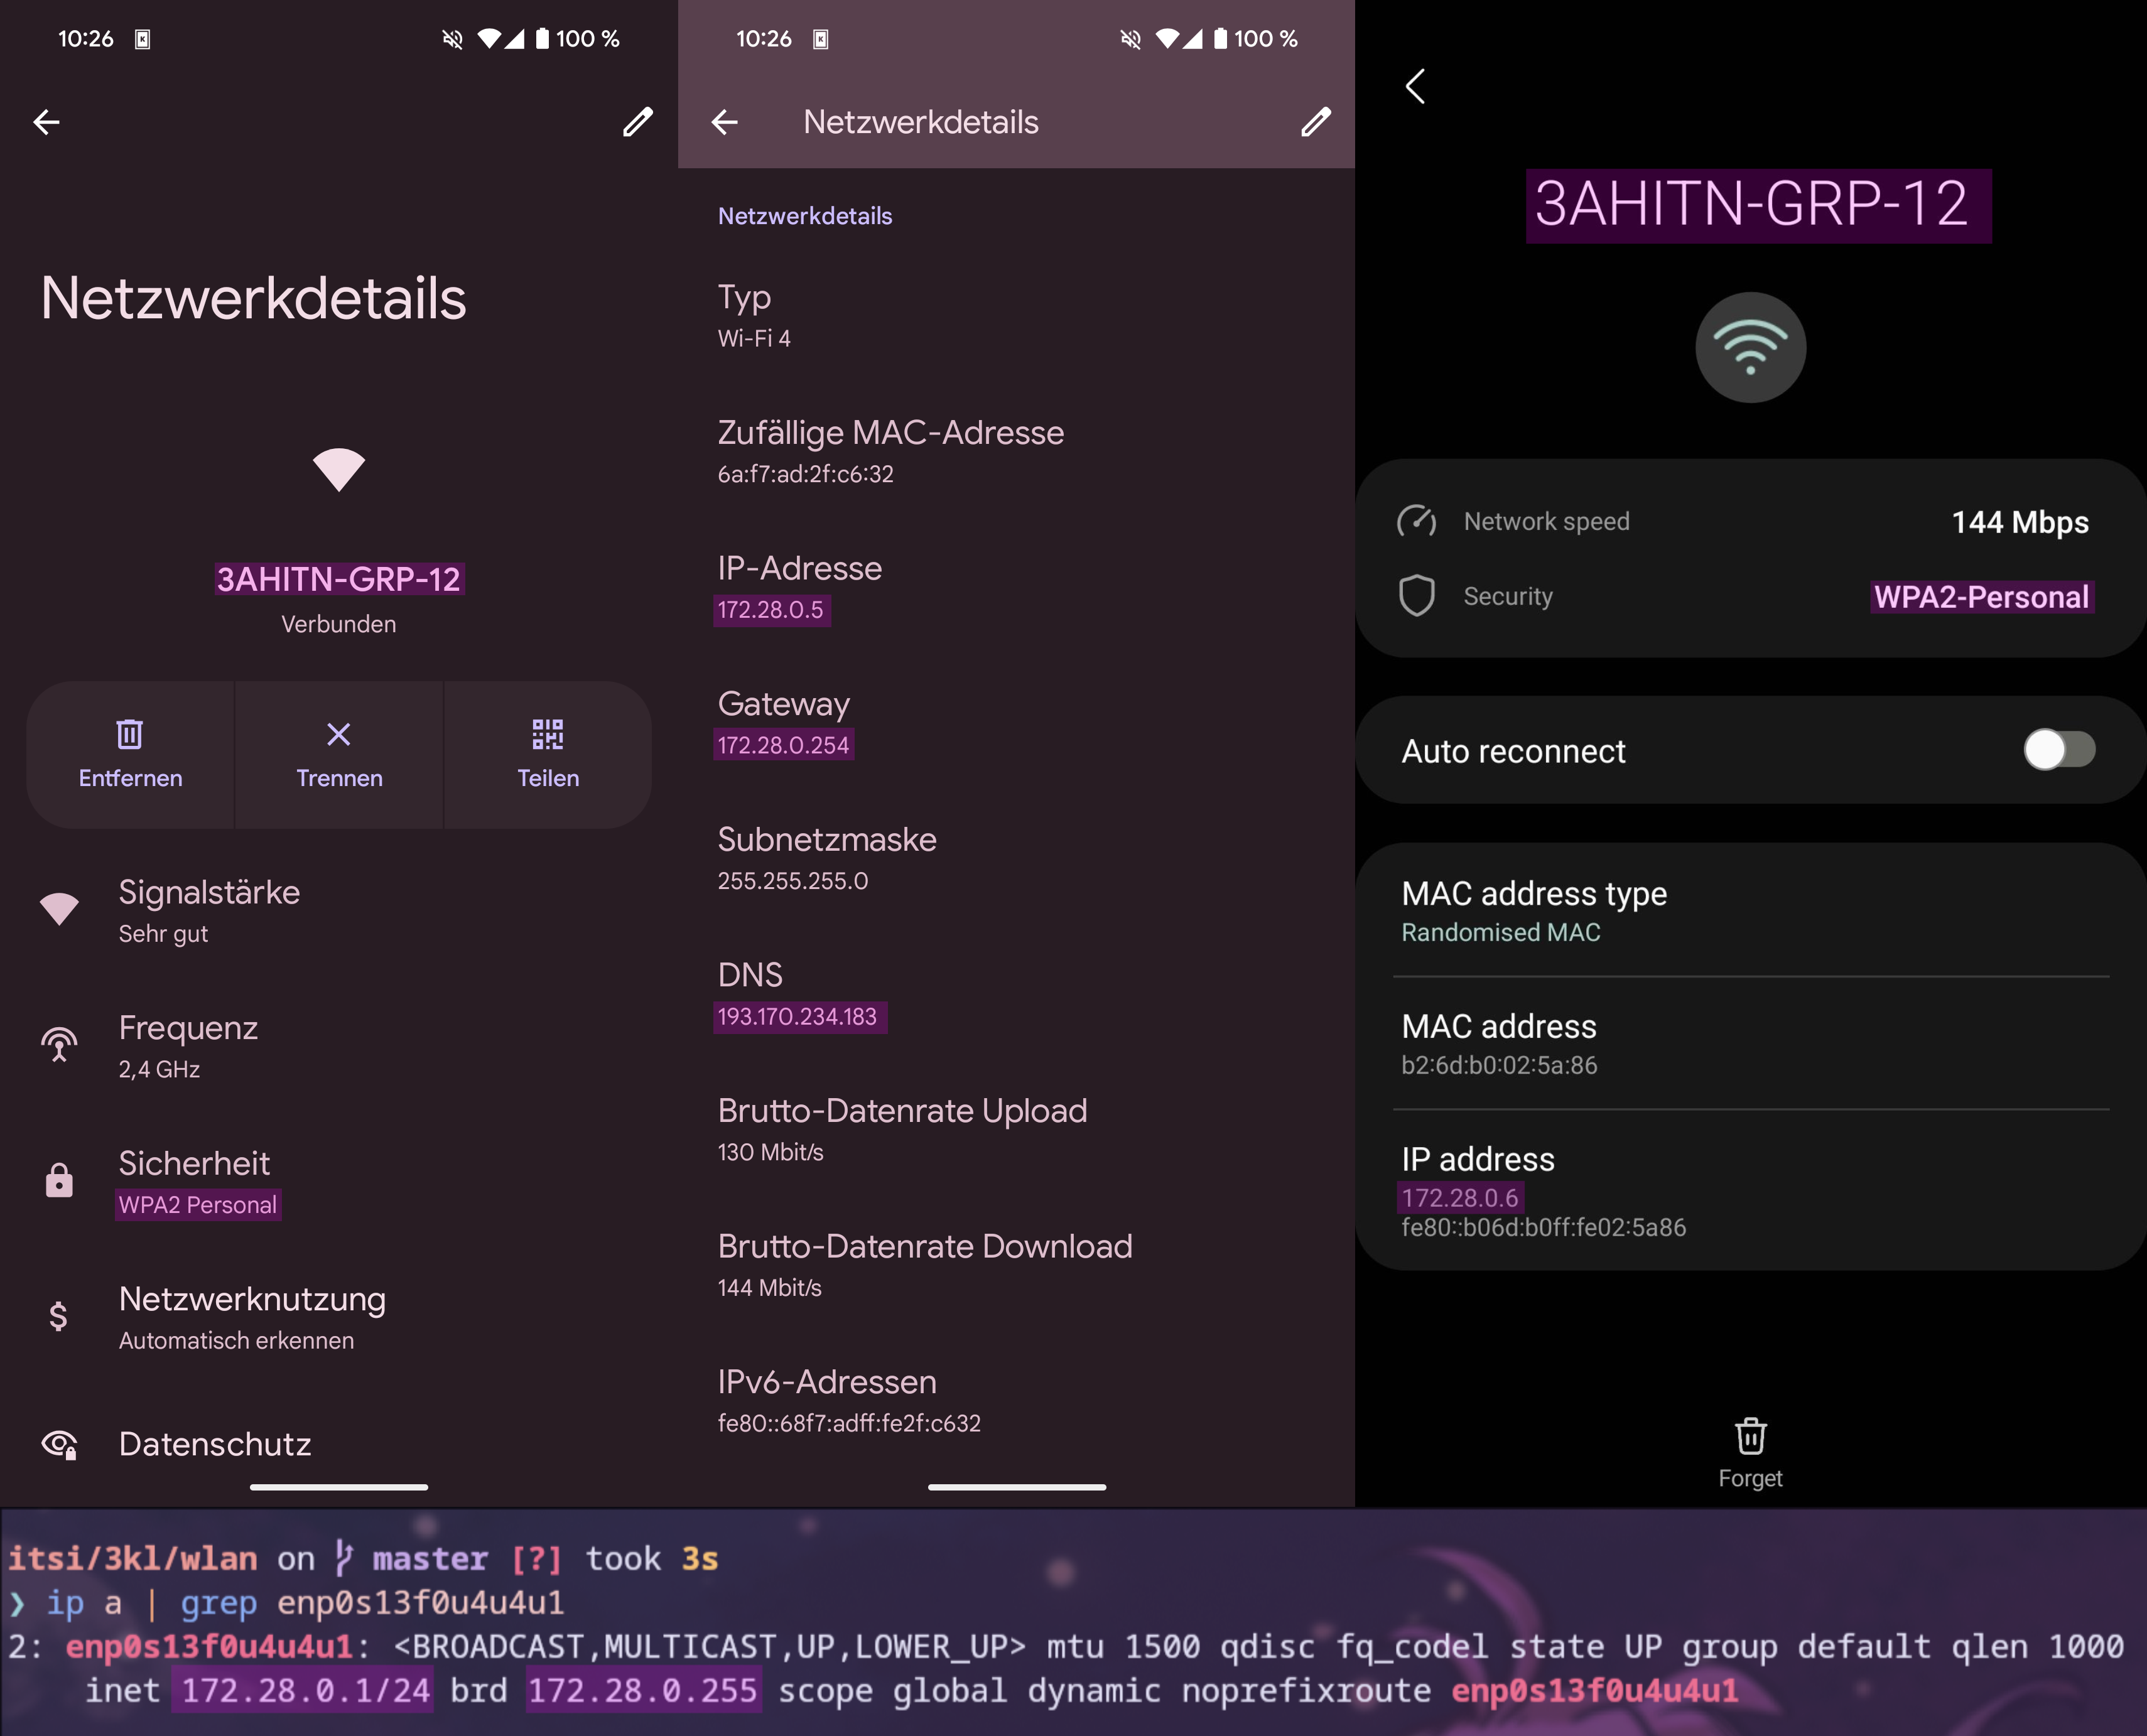
\includegraphics[scale=0.08]{images/phoenedge.png}
    \centering
    \caption{DHCP assigned addresses of the devices}
\end{figure}
\begin{figure}[!ht]
    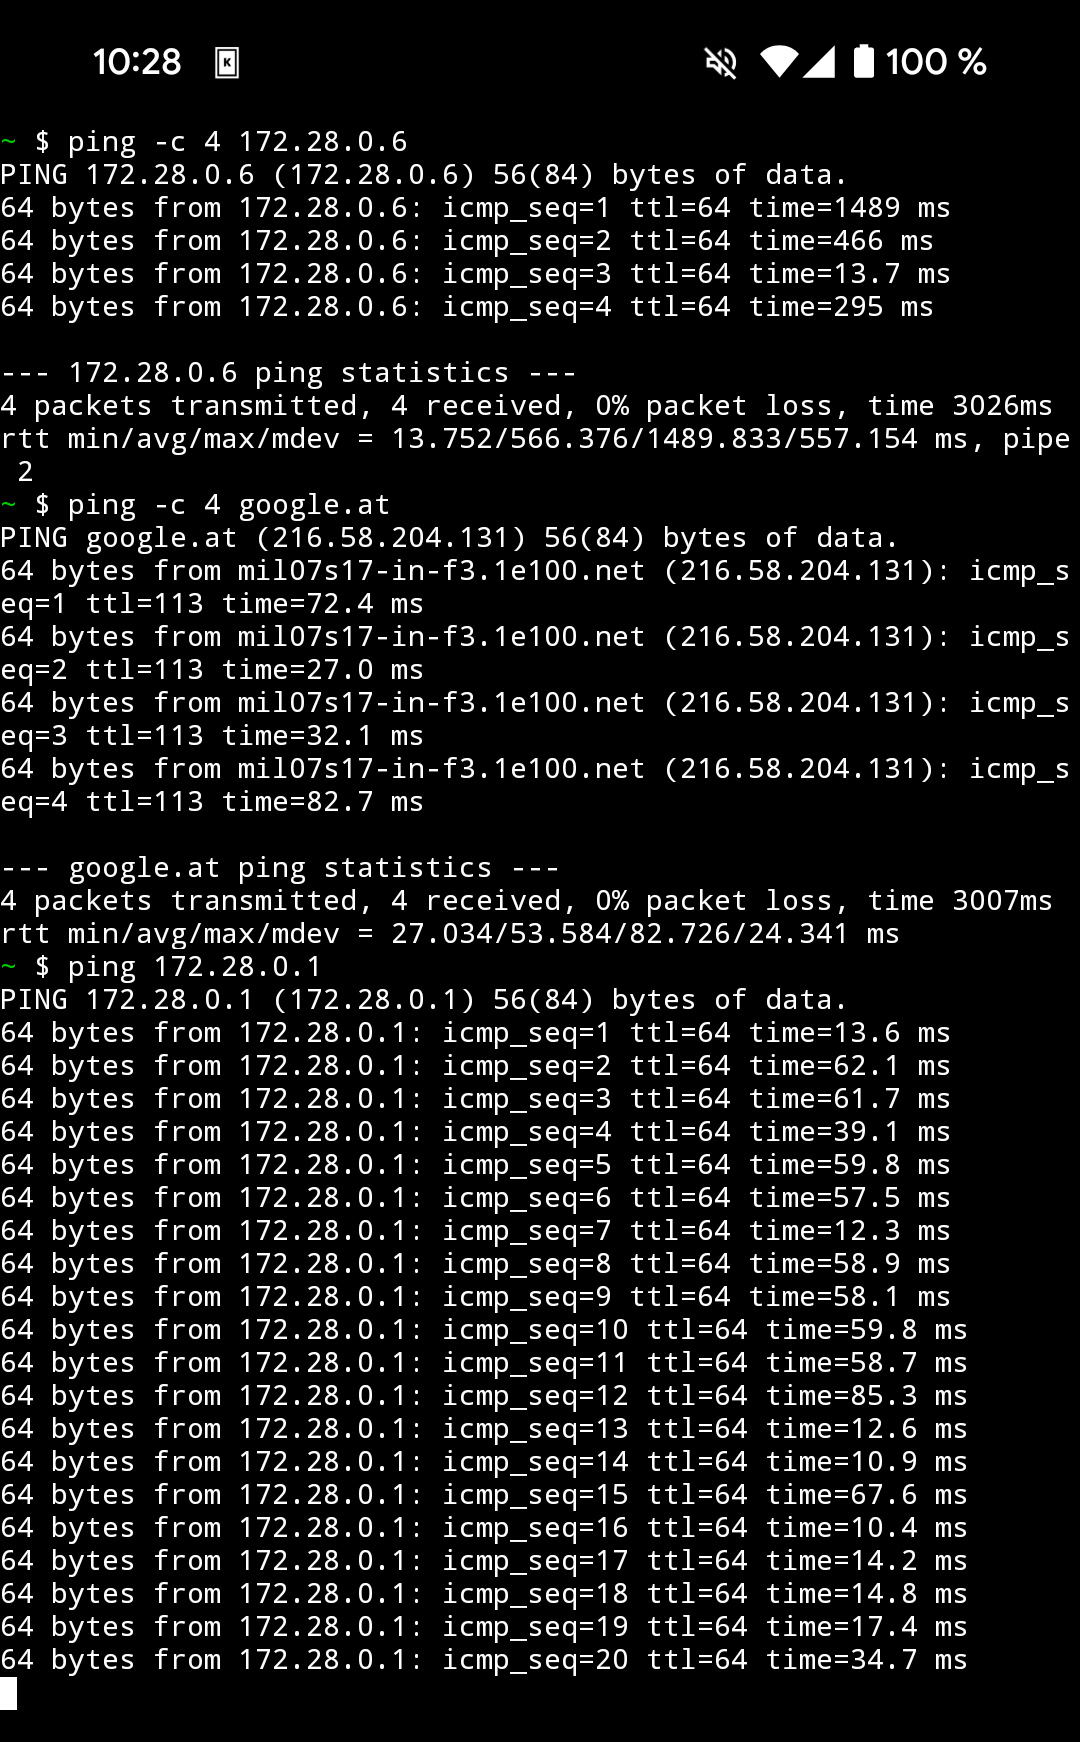
\includegraphics[scale=0.12]{images/conntest.png}
    \centering
    \caption{Testing the connectivity}
\end{figure} \newpage
\subsubsection{Access Point Isolation}
Access Point isolation is a feature that prevents wireless clients from communicating with other wireless clients; they cannot see each other nor ping each other. This is used for shared Wi-Fi networks, such as those found in airports. Having this feature enabled can break functionality like screen mirroring and controlling local IoT devices. In Figure 10, the topology of a home network, where a \texttt{Pixel 8a} device is used as a phone and \texttt{Steckdose} is a smart power plug, both connected to the access point, which has isolation turned on. As can be seen in Figure 11, the phone cannot ping the power plug due to the isolation, but control of the power plug is still possible since TP-Link made the great decision to provide it with internet access in the app \cite{noauthor_what_nodate}.
\begin{figure}[!ht]
    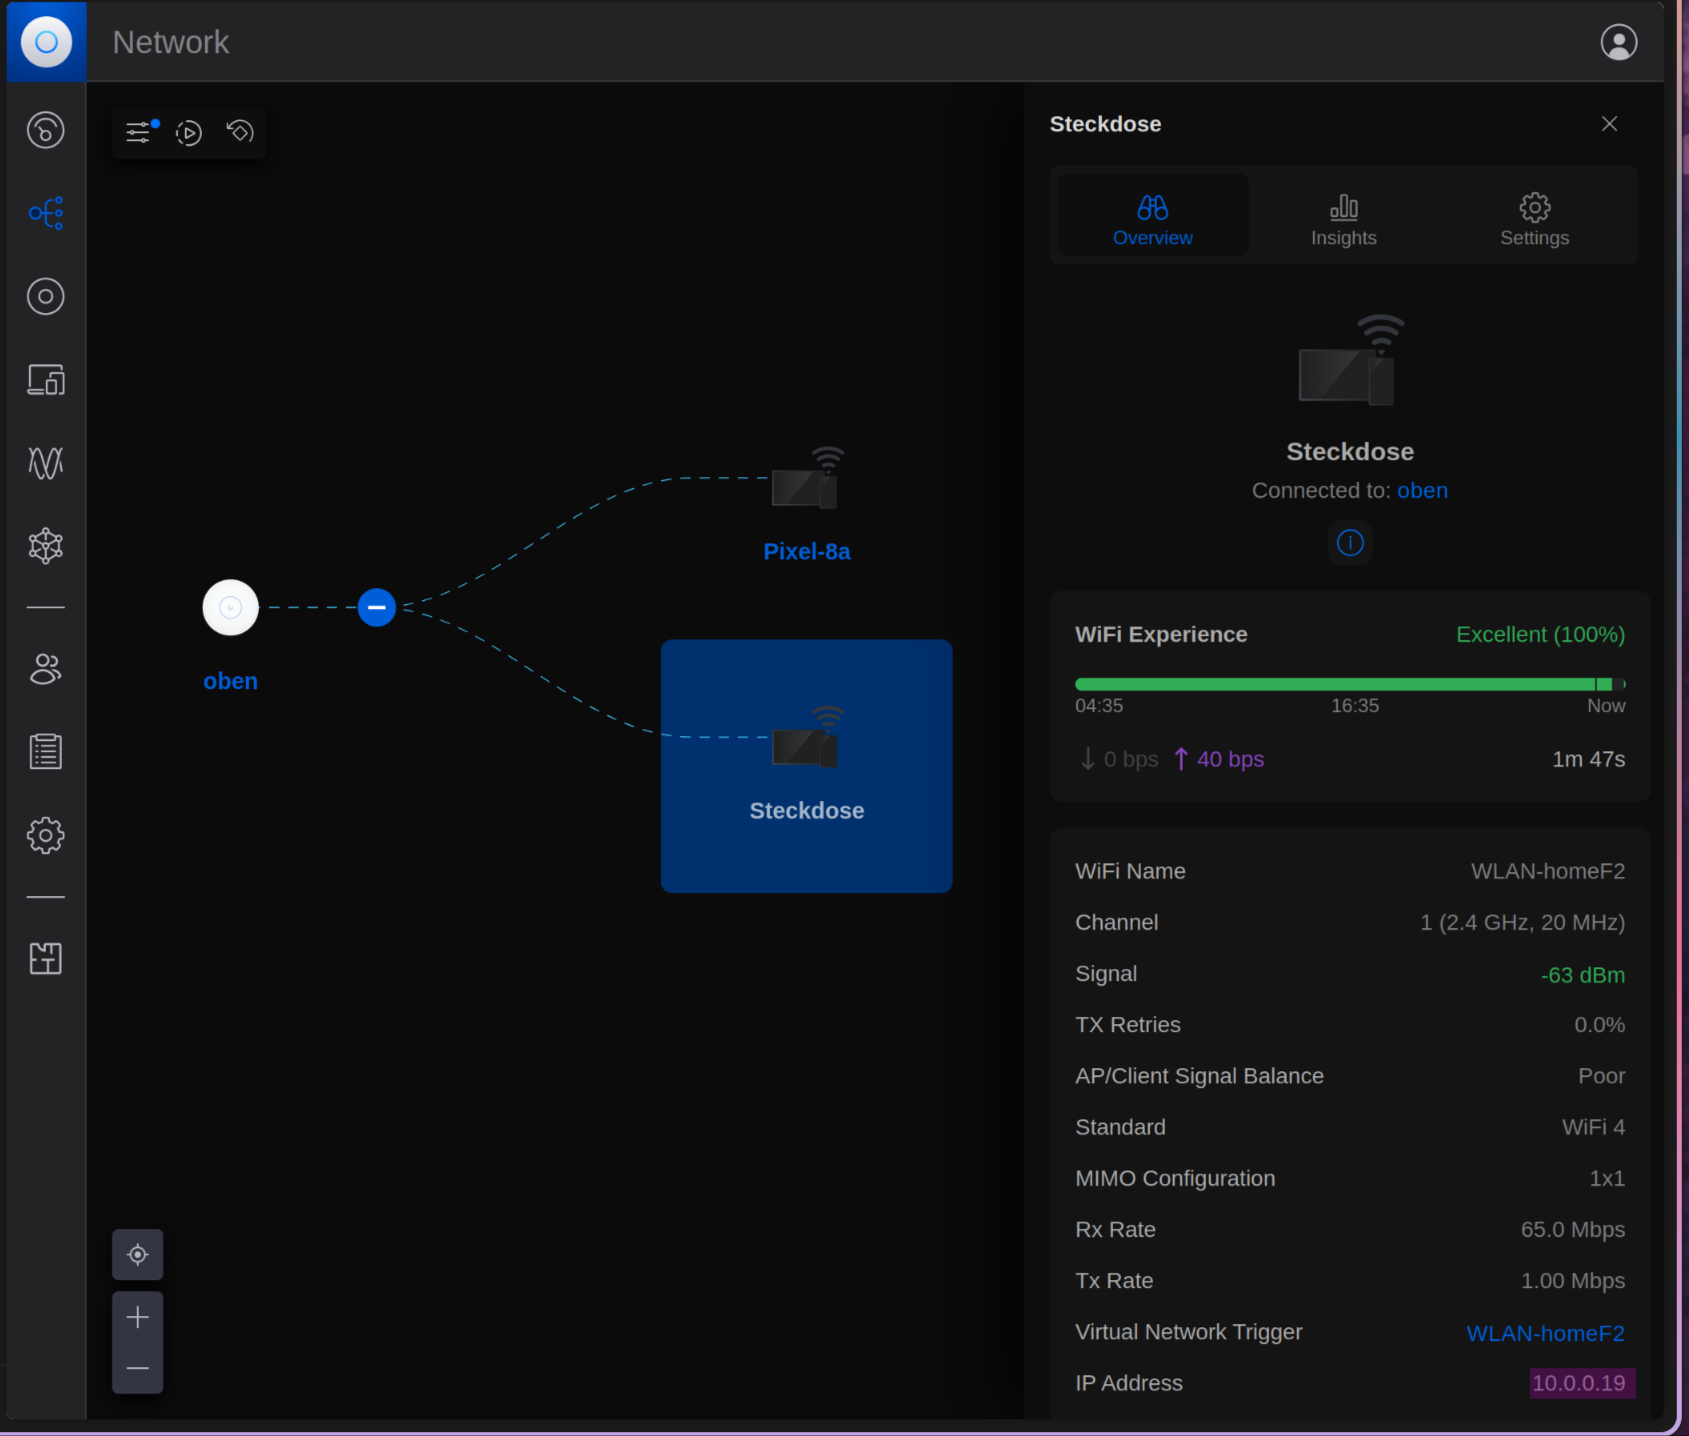
\includegraphics[scale=0.2]{images/steckdose_ip.png}
    \centering
    \caption{Showing the Topology for this example}
\end{figure}
\begin{figure}[!ht]
    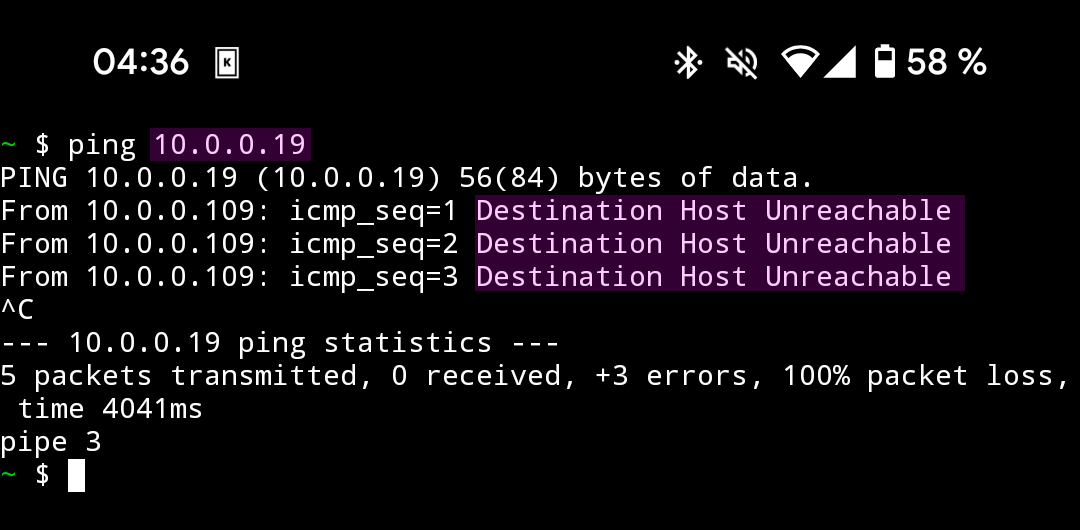
\includegraphics[scale=0.31]{images/steckdose_ping.png}
    \centering
    \caption{Trying to ping the Powerplug}
\end{figure} \newpage \nl
Isolation might sound like a feature that could prevent Wi-Fi hacking and sniffing handshakes, but as shown in Figure 12, even with isolation turned on, it does not stop an attacker from capturing all of the wireless traffic with a Wi-Fi adapter that supports monitoring mode, since the frames are transmitted through the air anyway and can therefore be stored.
\begin{figure}[!ht]
    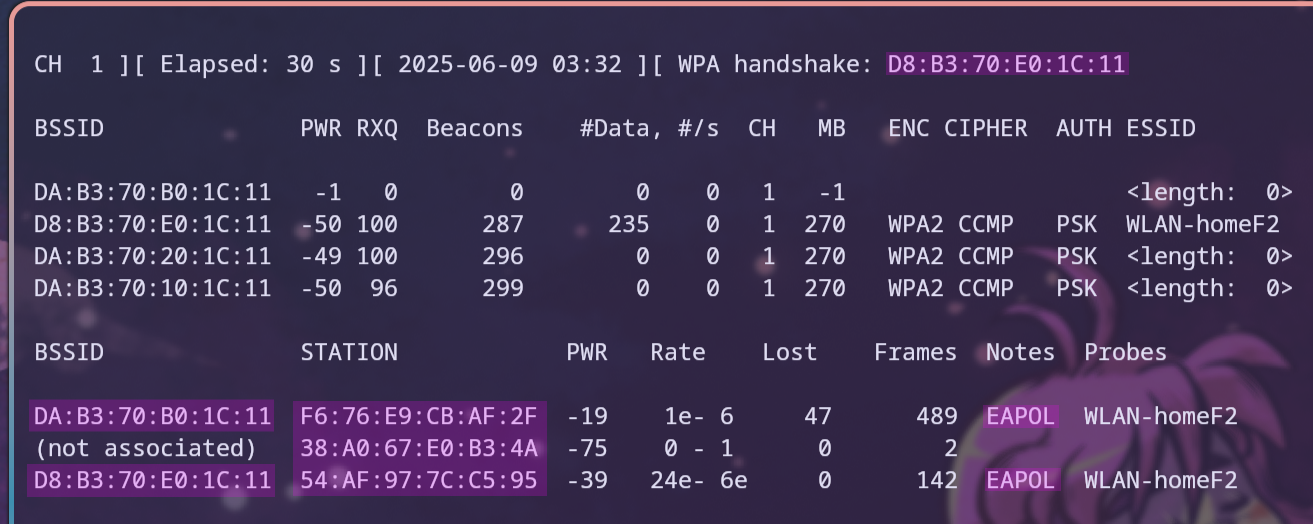
\includegraphics[scale=0.3]{images/islolateuseless.png}
    \centering
    \caption{Showing the Topology for this exmaple}
\end{figure} \newpage
\subsection{Attacking the Wi-Fi Network}
\subsubsection{Setting up the \texttt{Wi-Fi} Adapter}
To capture all frames, a Wi-Fi adapter with \texttt{Monitoring Mode} is required, which allows a computer with a \texttt{wireless network interface} to monitor all traffic on a wireless channel. Unlike \texttt{promiscuous mode}, which is also used for packet sniffing, monitor mode allows packets to be captured without having to associate with an access point or ad hoc network first. Monitor mode only applies to wireless networks, while \texttt{promiscuous mode} can be used on both wired and wireless networks \cite{noauthor_monitor_2024, noauthor_promiscuous_2025}. \nl
One of the most popular \texttt{Wi-Fi} chipsets that supports \texttt{Monitoring Mode} is the Realtek rtw88 series, for which drivers are available for Linux in this repository. For this exercise, a USB \texttt{Wi-Fi} adapter with the \texttt{RTL8821AU} chipset was used. The needed drivers were downloaded and installed following the instructions in the README from \url{https://github.com/lwfinger/rtw88}. \nl
To activate \texttt{Monitoring Mode}, the command \texttt{iw dev <interface> set type monitor} is used, and \texttt{iw dev <interface> info} can be used to verify the configuration. This command can also be used to check if the device supports \texttt{Monitoring Mode} or not, as can be seen in Figure 13. Additionally, the program \texttt{wifite} can be used to check whether the device supports \texttt{Monitoring Mode} or not, as showcased in Figure 14. \texttt{Wifite} is a Python script that automates wireless auditing using \texttt{aircrack-ng} tools \cite{noauthor_wifite_nodate}.
\begin{figure}[!ht]
    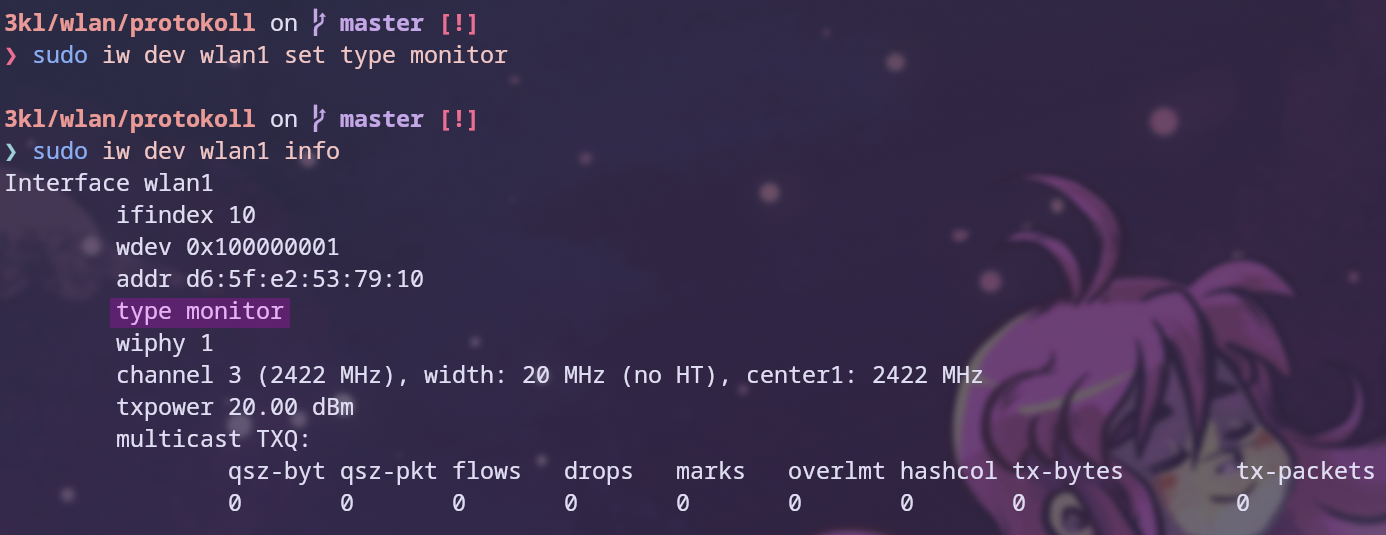
\includegraphics[scale=0.3]{images/iwdev.png}
    \centering
    \caption{Activating \texttt{Monitoring Mode} on the Interface via the \texttt{iw} command}
\end{figure}
\begin{figure}[!ht]
    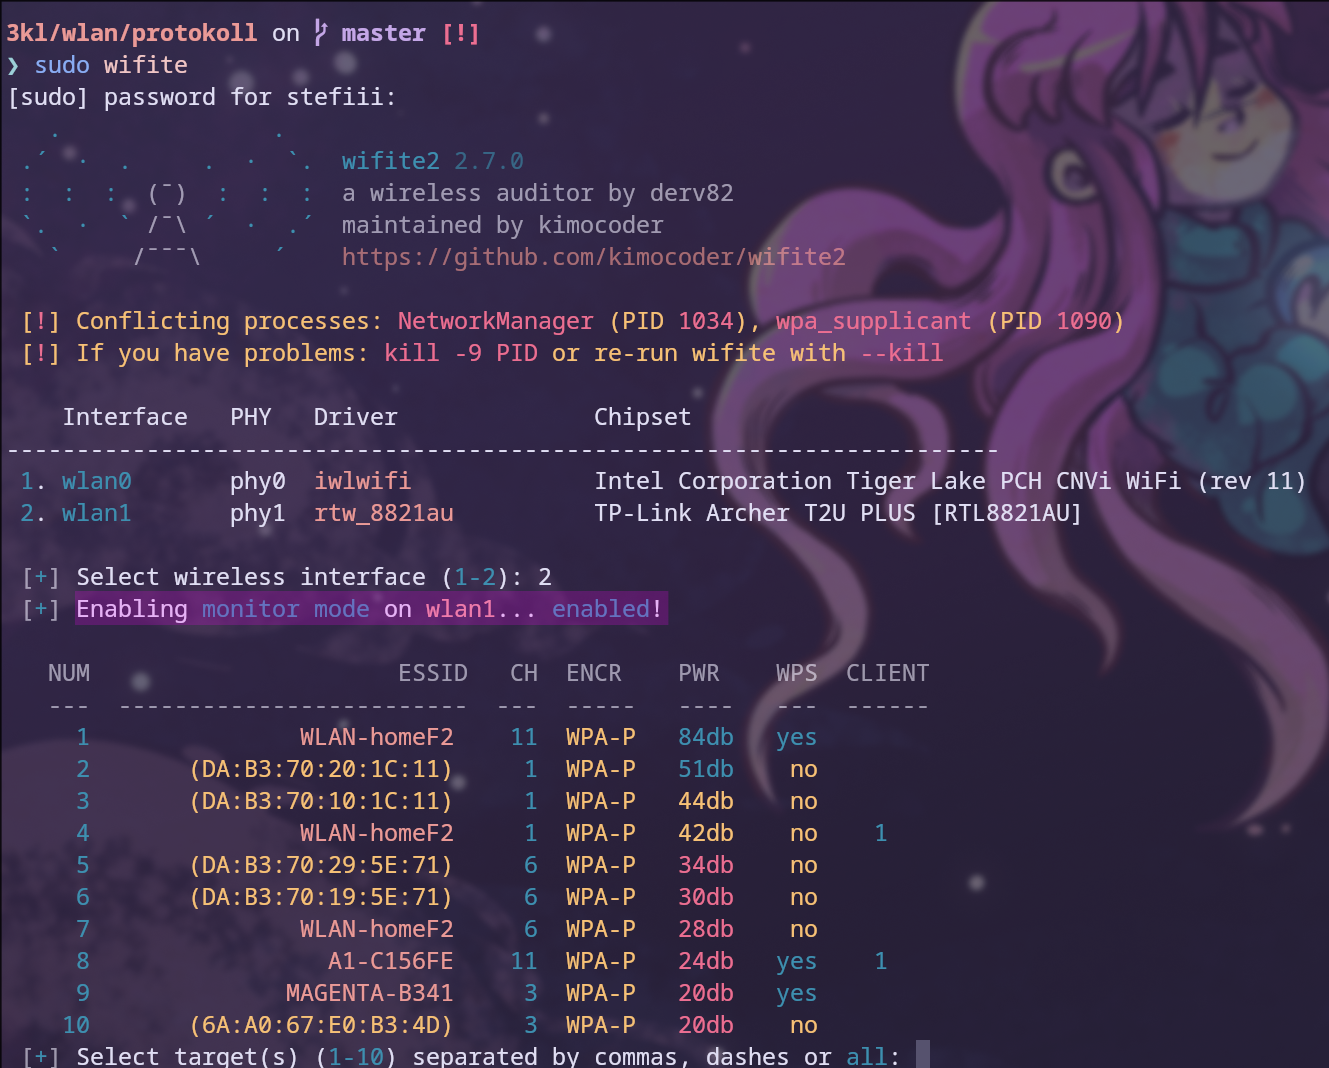
\includegraphics[scale=0.2]{images/wifite.png}
    \centering
    \caption{Activating \texttt{Monitoring Mode} on the Interface via \texttt{wifite}}
\end{figure} \newpage
\subsubsection{Starting the attack}
For the attack, the \texttt{Aircrack-ng} toolset is used to test the security of Wi-Fi networks. It supports monitoring, attacking, testing, cracking, and maintains patches for packet injection of Linux Wi-Fi drivers \cite{noauthor_main_nodate}. \nl
To get started, its \texttt{airmon-ng} script is used to enable monitor mode on the Wi-Fi adapter. The command used is \texttt{airmon-ng start <interface>}. It also checks for conflicting processes, such as network managers, and offers options to kill them to avoid interrupting the attack. However, I found that simply ignoring this warning has no effect if it's not the only Wi-Fi adapter in the system, as shown in Figure 15 \cite{noauthor_airmon-ng_nodate}.

\begin{figure}[!ht]
    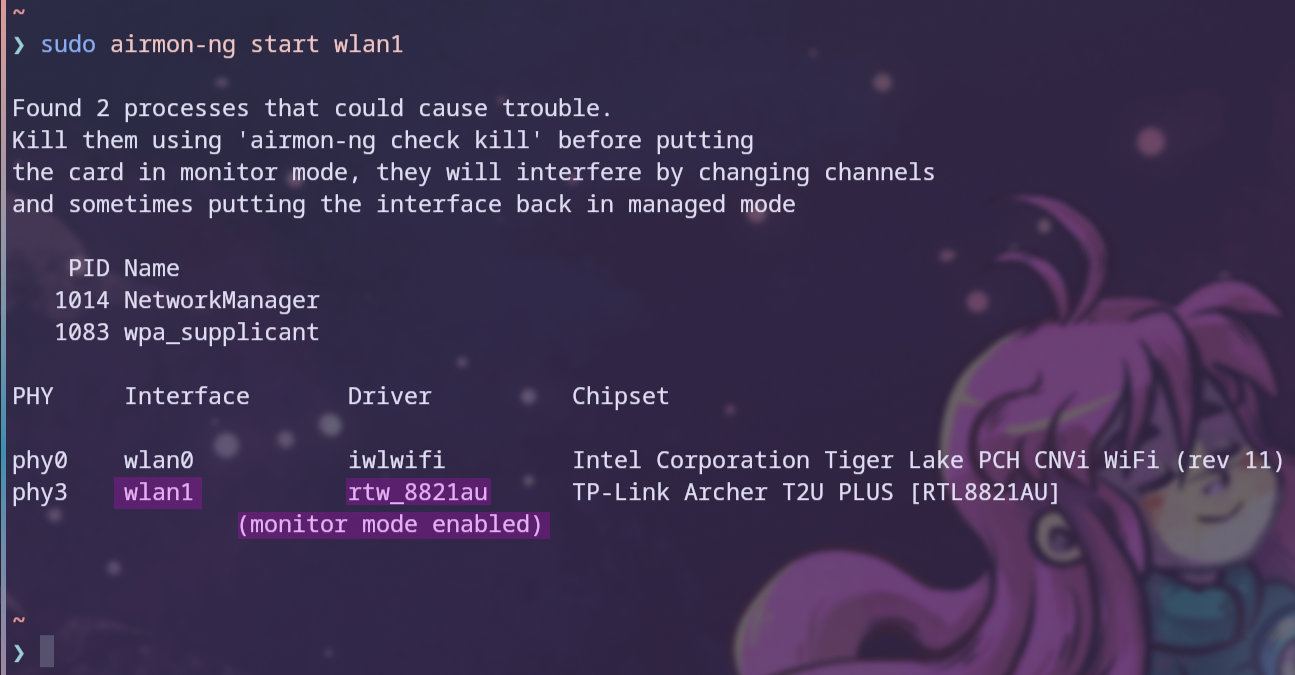
\includegraphics[scale=0.25]{images/airmon.png}
    \centering
    \caption{Activating \texttt{Monitoring Mode} on the Interface via \texttt{airmon-ng}}
\end{figure} \nl
To start the attack, the \texttt{BSSID}/MAC address of the access point, as well as the wireless channel, needs to be obtained. To do this, \texttt{airodump-ng} is used to capture raw \texttt{802.11} frames. \nl
To obtain all of that information, \texttt{airodump-ng <interface>} is used to get all the data from the detected active Wi-Fi networks and clients. Figure 16 shows the output, where the top half displays all of the detected access points while the bottom half shows the clients. It displays information such as \texttt{MAC Address}, signal strength, number of beacon and data frames, channel, encryption standard, cipher set, authentication method, and \texttt{ESSID} \cite{noauthor_airodump-ng_nodate}. \nl
\begin{figure}[!ht]
    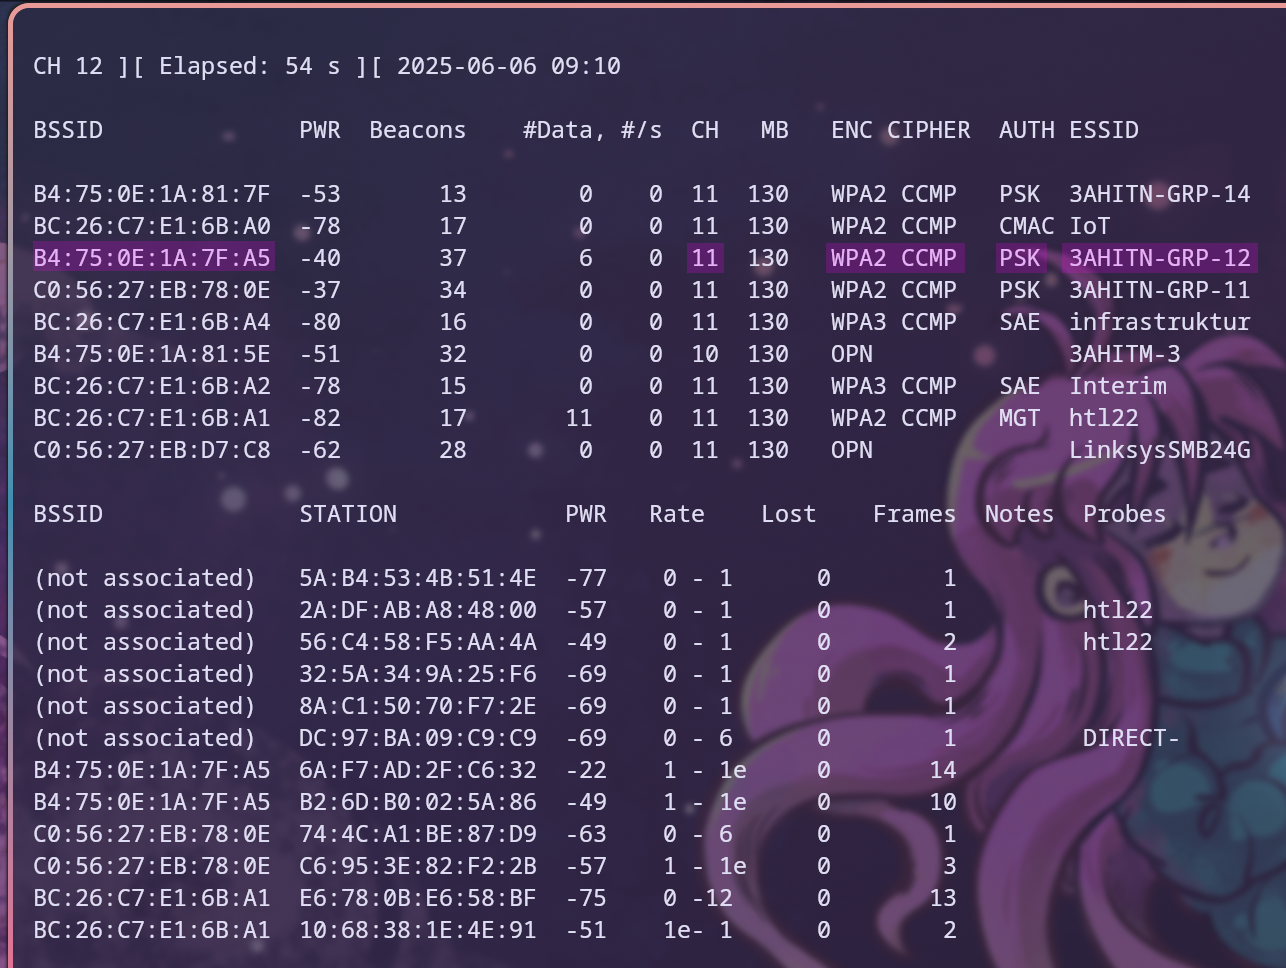
\includegraphics[scale=0.2]{images/aridodump1.png}
    \centering
    \caption{Gathering the needed information via \texttt{airodump-ng}}
\end{figure} \newpage \nl
With the information from Figure 16, we now know that the channel of the target Wi-Fi \texttt{3AHITN-GRP-12} is \texttt{11}, the \texttt{MAC Address} of the access point is \texttt{B4:75:0E:1A:7F:A5}, and that it uses \texttt{WPA2-Personal} with the \texttt{CCMP} cipher set. A new command can be used that specifies the correct channel and \texttt{BSSID}, and also writes the captured data to files using the \texttt{-w} option. \nl
The command used was \texttt{sudo airodump-ng -c 11 --bssid B4:75:0E:1A:7F:A5 -w thing wlan1}, where the \texttt{-c} option sets the channel to use, the \texttt{--bssid} option specifies the BSSID of the desired access point, the \texttt{-w} option writes the capture to files starting with the name \texttt{thing}, and finally, the interface to use is specified, which in this case is \texttt{wlan1} \cite{noauthor_airodump-ng_nodate}. \nl
Now, only the desired access point is captured, and all its clients can be seen in the bottom half of the screen, as shown in Figure 17.
\begin{figure}[!ht]
    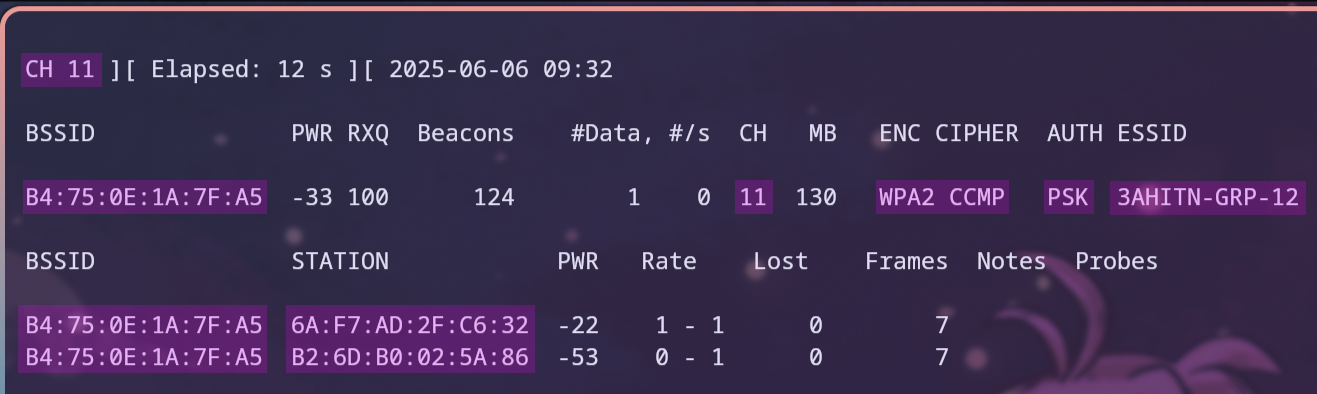
\includegraphics[scale=0.32]{images/airodump2.png}
    \centering
    \caption{Capturing frames from and to the target access point}
\end{figure}\nl
\subsubsection{Sending Deauthentication Frames}
To capture a 4-Way WPA2 handshake, there are two options: wait for a client to connect or send a \texttt{deauthentication} frame with the \texttt{MAC Address} of a client to disconnect it. This can easily be captured using packet sniffing, and if the client has automatic reconnect enabled, the handshake can be captured \cite{noauthor_wi-fi_2025}. \nl
This is called a deauthentication attack, which is a type of denial-of-service attack, as it actively stops the connection of a client. This method can also be used on the entire network if a tool like \texttt{aireplay-ng} is used to send the frame with the \texttt{MAC Address} of all the clients, allowing the attacker to take down the entire Wi-Fi network. This is useful for either an Evil Twin attack or, as in our case, a password attack to capture the handshake for decryption \cite{noauthor_wi-fi_2025, noauthor_aireplay-ng_nodate}. \nl
To deauthenticate one of the clients, the following command was used:\nl
\texttt{sudo aireplay-ng -0 1 -a B4:75:0E:1A:7F:A5 -c 6A:F7:AD:2F:C6:32 wlan1}.\nl
This uses \texttt{aireplay-ng} to generate traffic for later use with \texttt{aircrack-ng}. One of its uses is to send \texttt{deauthentication frames}. The first option of the above command is \texttt{-0} with \texttt{1} as the value. Here, \texttt{-0} means deauthentication, and the number sets the number of \texttt{deauthentication frames} to send. If that value is \texttt{0}, \texttt{deauthentication frames} are sent until the program is exited. In this case, only one is sent to hopefully prompt the client to reconnect. Multiple frames are only necessary if the goal is to keep the connection down for an Evil Twin attack or just a denial-of-service attack in general. The \texttt{-a} option is used to specify the \texttt{MAC Address} of the access point to which the \texttt{deauthentication frame} will be sent, while \texttt{-c} is the client whose MAC address will be spoofed in the packet to disconnect them. If the \texttt{-c} option is not set, \texttt{aireplay-ng} will try to disconnect all clients by sending the \texttt{deauthentication frames} to the brodcast, which is a more effective denial-of-service method. However, as my goal is only to get one handshake, I chose a specific client. Disconnecting multiple devices is not wise if the goal is only to capture one handshake, as it could raise suspicion that someone is trying to perform a DoS attack on the Wi-Fi network. The output of the command can be examined in Figure 18 on the next page. \cite{noauthor_deauthentication_nodate}\newpage
\begin{figure}[!ht]
    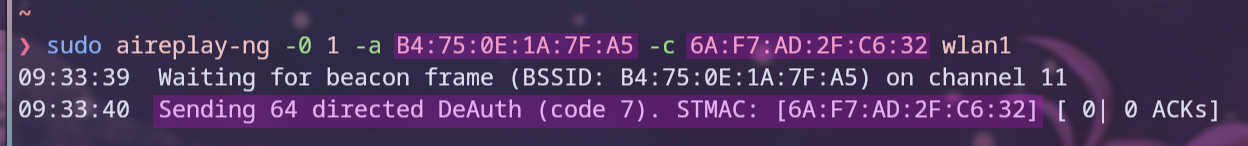
\includegraphics[scale=0.32]{images/deauth.png}
    \centering
    \caption{Sending one \texttt{deauthentication frame} as the targeted client to the access point}
\end{figure}\nl
To filter for \texttt{deauthentication frames} in Wireshark, the following filter can be used: \nl
\texttt{(wlan.fc.type eq 0) \&\& (wlan.fc.type\_subtype eq 12)} \nl
The part in the first parentheses filters only for \texttt{Management frames}, and the second one checks if the \texttt{Frame Type/Subtype} is equal to 12, which is the code for a \texttt{deauthentication frame} \cite{writer_analyzing_2018}. \nl
Looking at the frame itself, as shown in Figure 19, nothing special or complicated is going on; it is just the frame that \texttt{aireplay-ng} created, and it contains the receiver, destination, transmitter, source address, and BSSID.
\begin{figure}[!ht]
    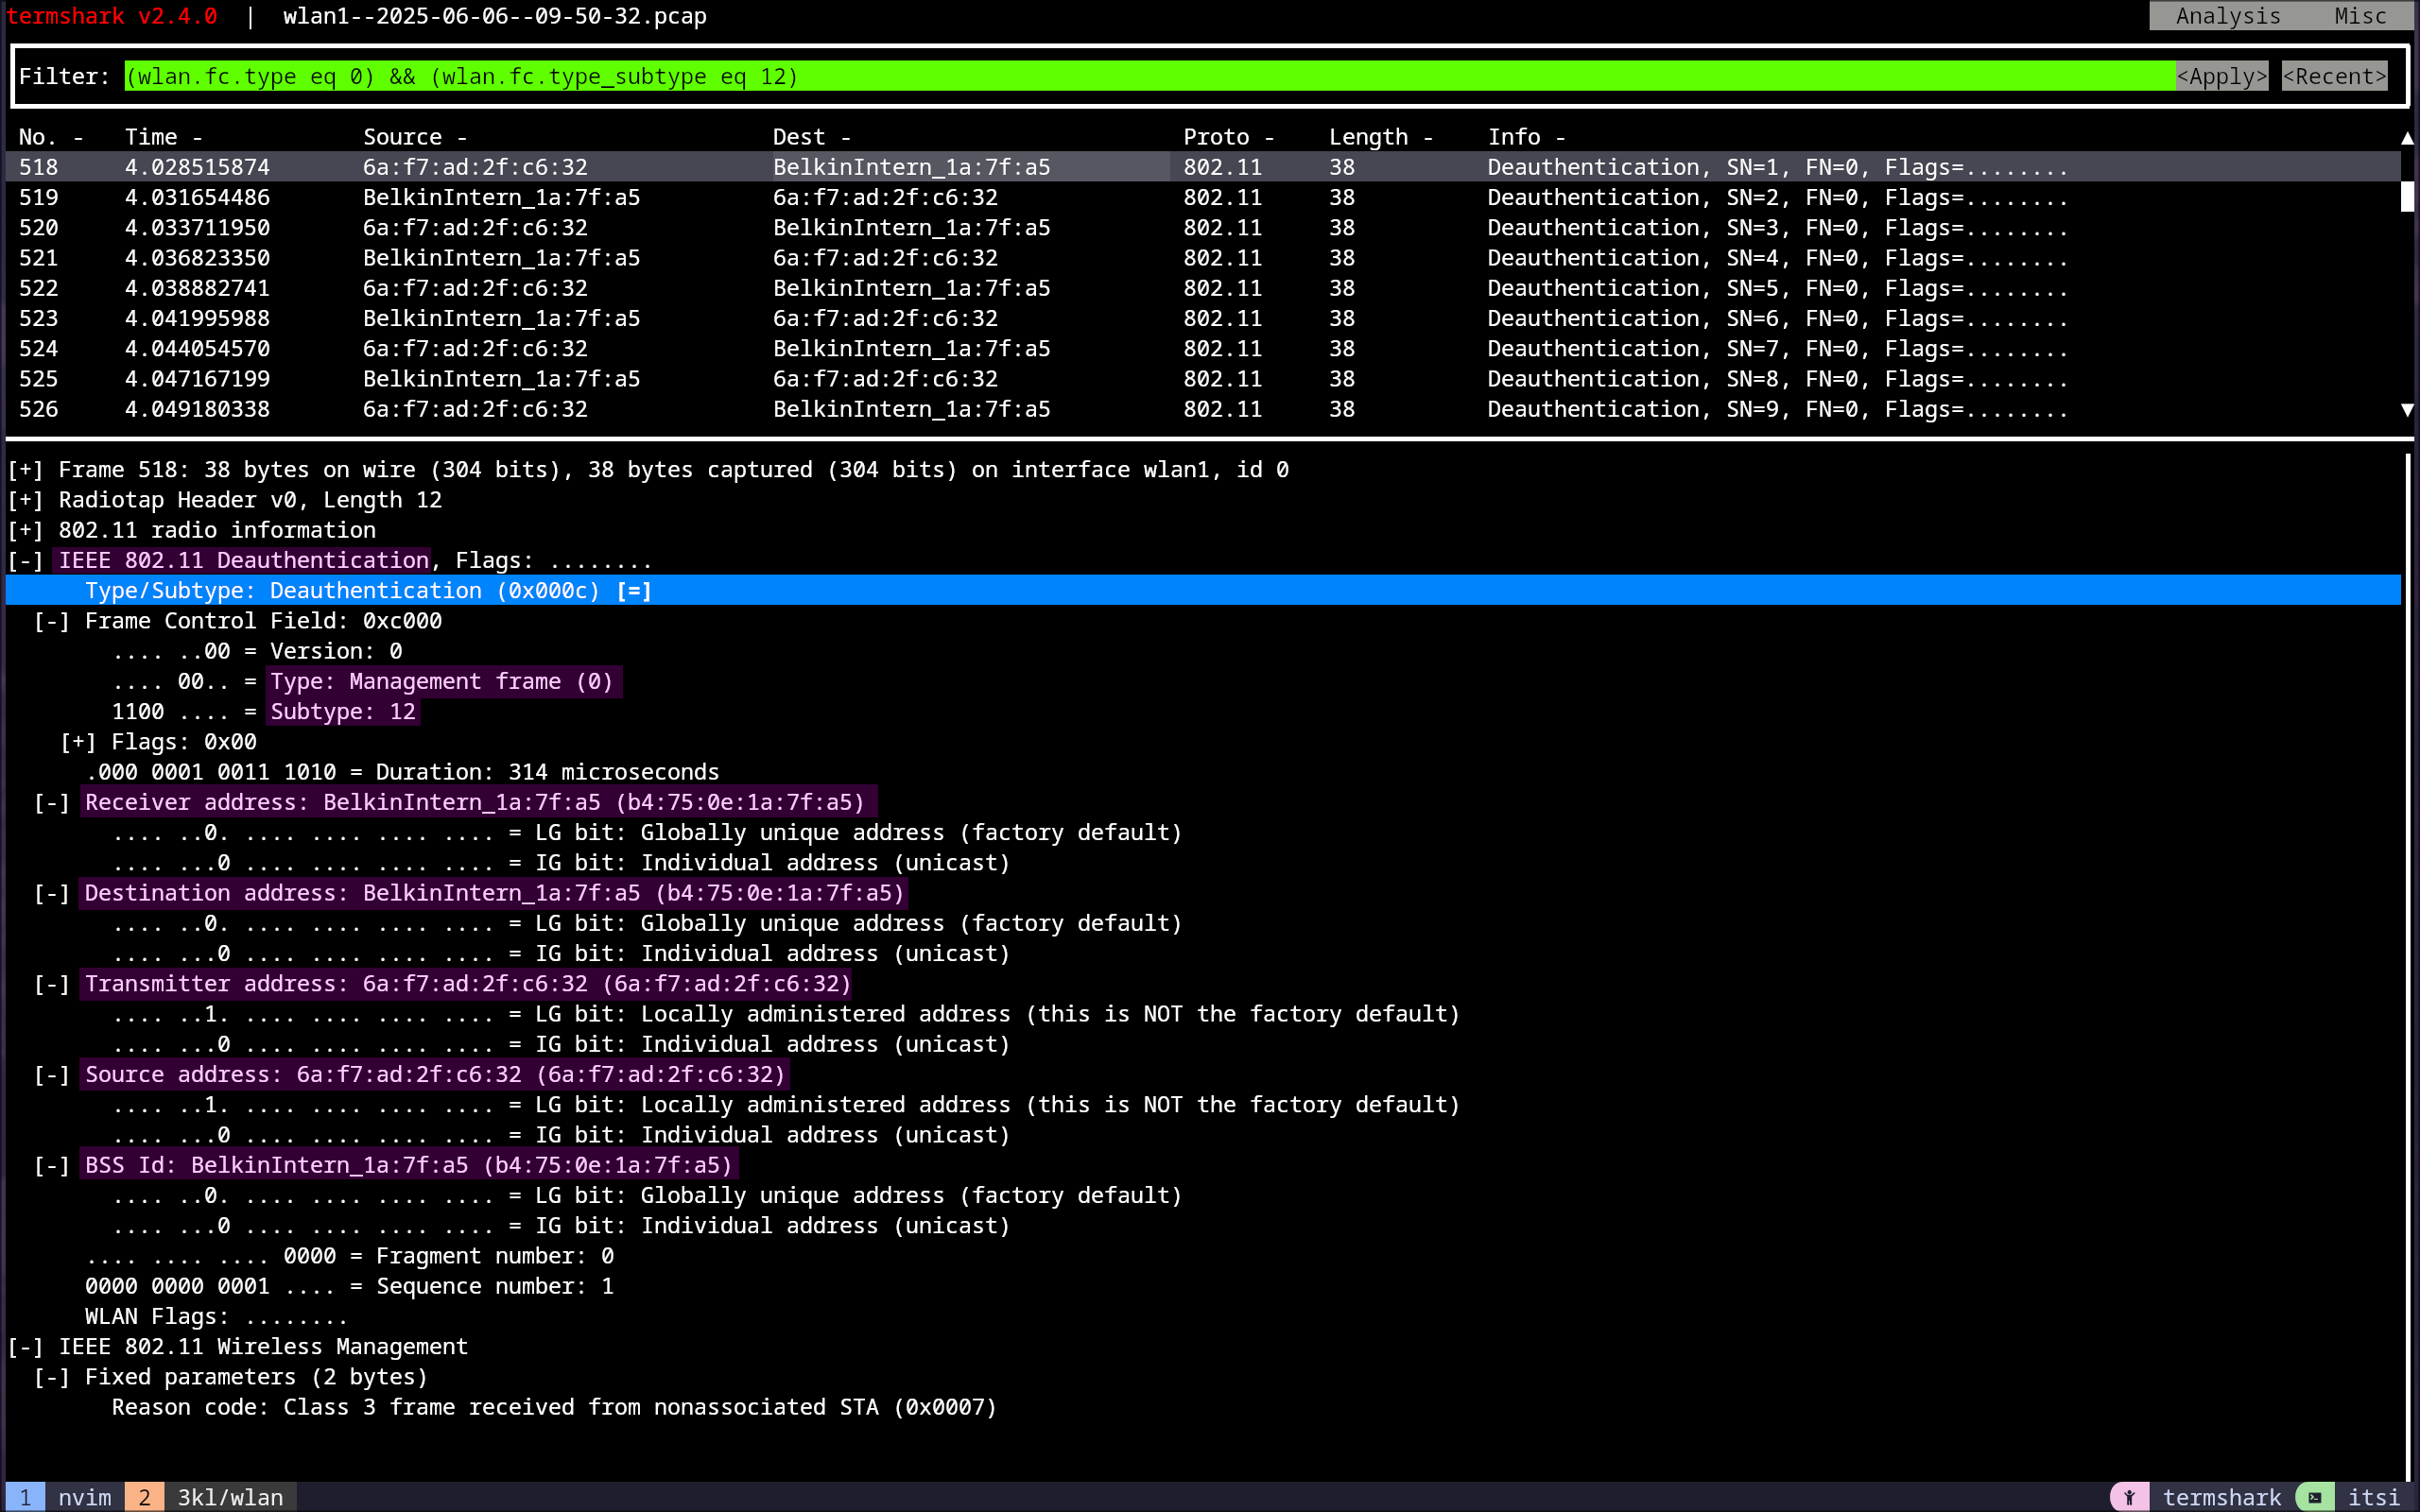
\includegraphics[scale=0.18]{images/deauth frame.png}
    \centering
    \caption[Viewing a \texttt{deauthentication frame} in Wireshark]{Viewing a \texttt{deauthentication frame} in Wireshark \footnotemark }
\end{figure}\nl
\footnotetext{I know this is not Wireshark, but I felt that writing "Termshark" instead would sound awkward. However, it is essentially the same program, just in the terminal and with Vim motions. Additionally, for the next exercise, it will be themed to look better and present captured frames in the cleanest way possible.}
Now that the client has been disconnected, if we look back at the running capture from before, we can see that once a handshake has occurred, it is printed out in the first line for which \texttt{BSSID} it was captured, as well as in the \texttt{Notes} section of the client, which gets populated with the \texttt{EAPOL} value. \texttt{EAPOL} stands for \texttt{Extensible Authentication Protocol over LANs (IEEE P802.1X-REV)} and is the protocol over which the WPA2 handshake is carried out, as stated on page 7 in the Definitions section of the \texttt{802.11i (WPA2)} standard \cite{noauthor_ieee_2021}. \nl
This can be examined in Figure 20 on the next page; however, this screenshot was taken on a different day in a different environment. When I first took the screenshot, I overlooked that the message had popped up, and therefore I repeated parts of the exercise on my home network to gather the screenshot.
\begin{figure}[!ht]
    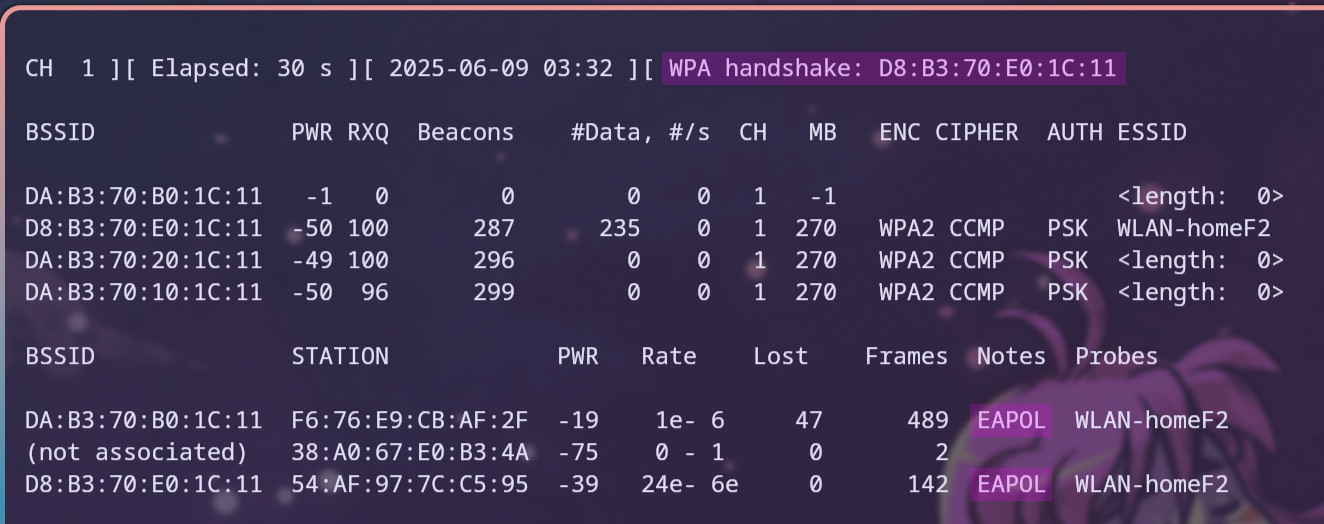
\includegraphics[scale=0.32]{images/thing.png}
    \centering
    \caption{Highlighting the visual confirmation of the captured handshake}
\end{figure}
\subsection{Analyzing the 4-Way Handshake in Wireshark}
Now that the handshake has been captured, it's time to analyze the captured handshake in Wireshark and decrypt it to obtain the password. \nl
To filter for the handshake, the following filter was used: \nl
\texttt{eapol \&\& !eap} \nl
This filter only displays frames with \texttt{EAPOL}, which are responsible for authentication, and excludes frames that contain \texttt{EAP} (Extensible Authentication Protocol (IETF RFC 3748)), which is only used for WPA2-Enterprise and therefore not relevant for now.
\subsubsection{EAPOL Frame Fields}
As stated in section 4.2.3, \texttt{EAPOL} is used to carry authentication data between the supplicant and the authenticator, resulting in the exchange of cryptographic keys and synchronization of the security association state. To understand a breakdown of the 4 frames of the handshake, the relevant fields of an \texttt{EAPOL} frame will be explained \cite{noauthor_ieee_2021}. \nl
Figure 21 shows the parts of an \texttt{EAPOL frame} and is a remake of the graphic found on page 78 of the WPA2 specification \cite{noauthor_ieee_2021}. \nl
\begin{figure}[!ht]
    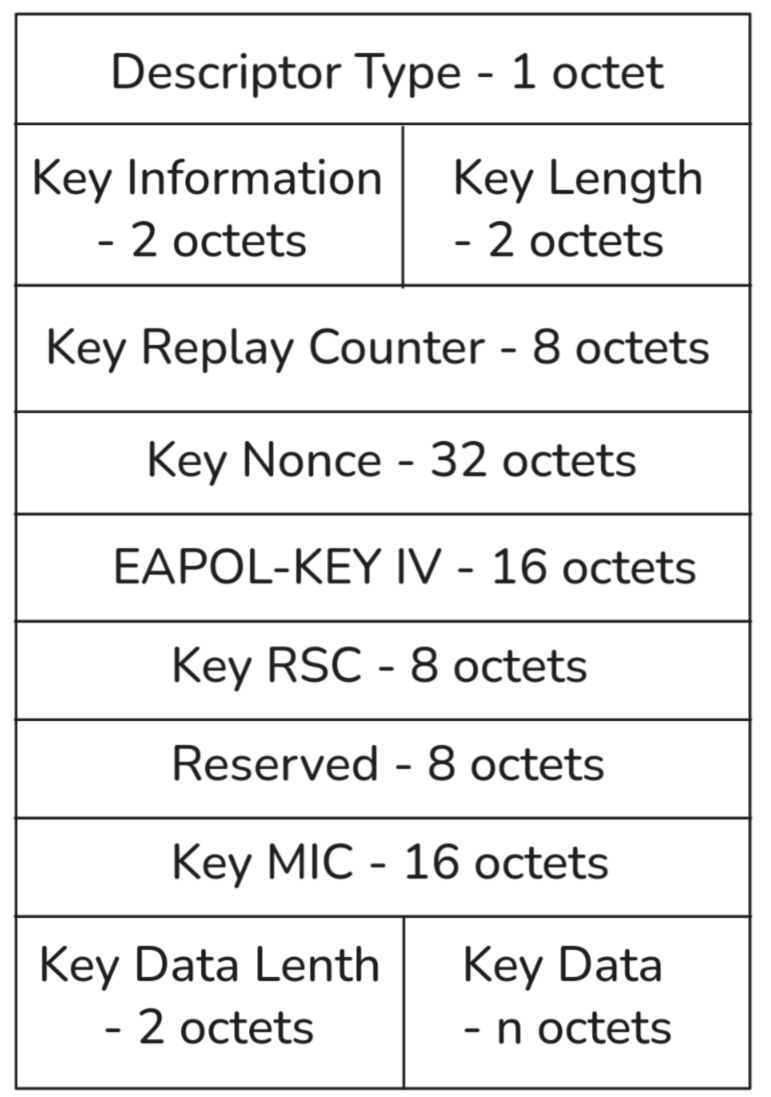
\includegraphics[scale=0.18]{images/eapolframe.png}
    \centering
    \caption{Layout of an \texttt{EAPOL frame}}
\end{figure} \newpage

\paragraph{Descriptor Type} \nl
This field stores the type of the key, which contains the used cipher suite; for example, it could be \texttt{AES} \cite{noauthor_ieee_2021}.
\paragraph{Key Information} \nl
The 2 octets of this field specify characteristics of the key, which could include \texttt{Error, Key MIC, Key ACK}, etc. The full chart for this can be found in Figure 43—Key Information bit layout on page 78 of the specification \cite{noauthor_ieee_2021}.
\paragraph{Key Length} \nl
An unsigned binary number defining the length of the pairwise temporal key to configure into IEEE 802.11. The value varies per used cipher suite and is shown in Table 20—Cipher suite key lengths on page 79 of the specification \cite{noauthor_ieee_2021}.
\paragraph{Key Replay Counter} \nl
Acts as a sequence number and is initialized as 0 when the \texttt{PMK} is established. The supplicant uses it to detect replayed frames, and the authenticator increments the number on each successive \texttt{EAPOL-Key frame}. When replying, the supplicant shall use the counter field from the last valid frame received from the authenticator, who shall use the value to silently discard invalid frames \cite{noauthor_ieee_2021}.
\paragraph{Key Nonce} \nl
Conveys the ANonce, which is just a random number used for the authentication from the authenticator and the SNonce from the supplicant. It may contain 0 if a nonce is not required to be sent \cite{noauthor_ieee_2021}.
\paragraph{Key RSC} \nl
Contains the receive sequence counter (RSC) for the GTK being installed in WPA2. It is used in Message 3 of the 4-Way Handshake and Message 1 of the Group Key Handshake, where it is used to synchronize the IEEE 802.11 replay state \cite{noauthor_ieee_2021}.
\paragraph{Key MIC} \nl
The \texttt{Key MIC} is a \texttt{MIC (Message Integrity Code)} calculated from the \texttt{Key Descriptor Value} and \texttt{Key Data Field} \cite{noauthor_ieee_2021}.
\paragraph{Key Data Length} \nl
Represents the length of the encrypted key data field \cite{noauthor_ieee_2021}.
\paragraph{Key Data} \nl
A variable-length field that is used to include any additional data required for the key exchange that is not included in the fixed fields of the EAPOL-Key frame \cite{noauthor_ieee_2021}. \newpage
\subsubsection{4-Way Handshake Message 1}
The authenticator sends an \texttt{ANonce} to the client, which is a pseudo-random number generated by it. This \texttt{ANonce} will be used by the supplicant to generate its \texttt{SNonce}. This can be seen in Figure 22 below, where the replay counter has also been incremented due to the \texttt{R} flag being set in the Wi-Fi header, since the first packet was dropped and is being replayed \cite{noauthor_ieee_2016-1, admin_4-way_2019}.
\begin{figure}[!ht]
    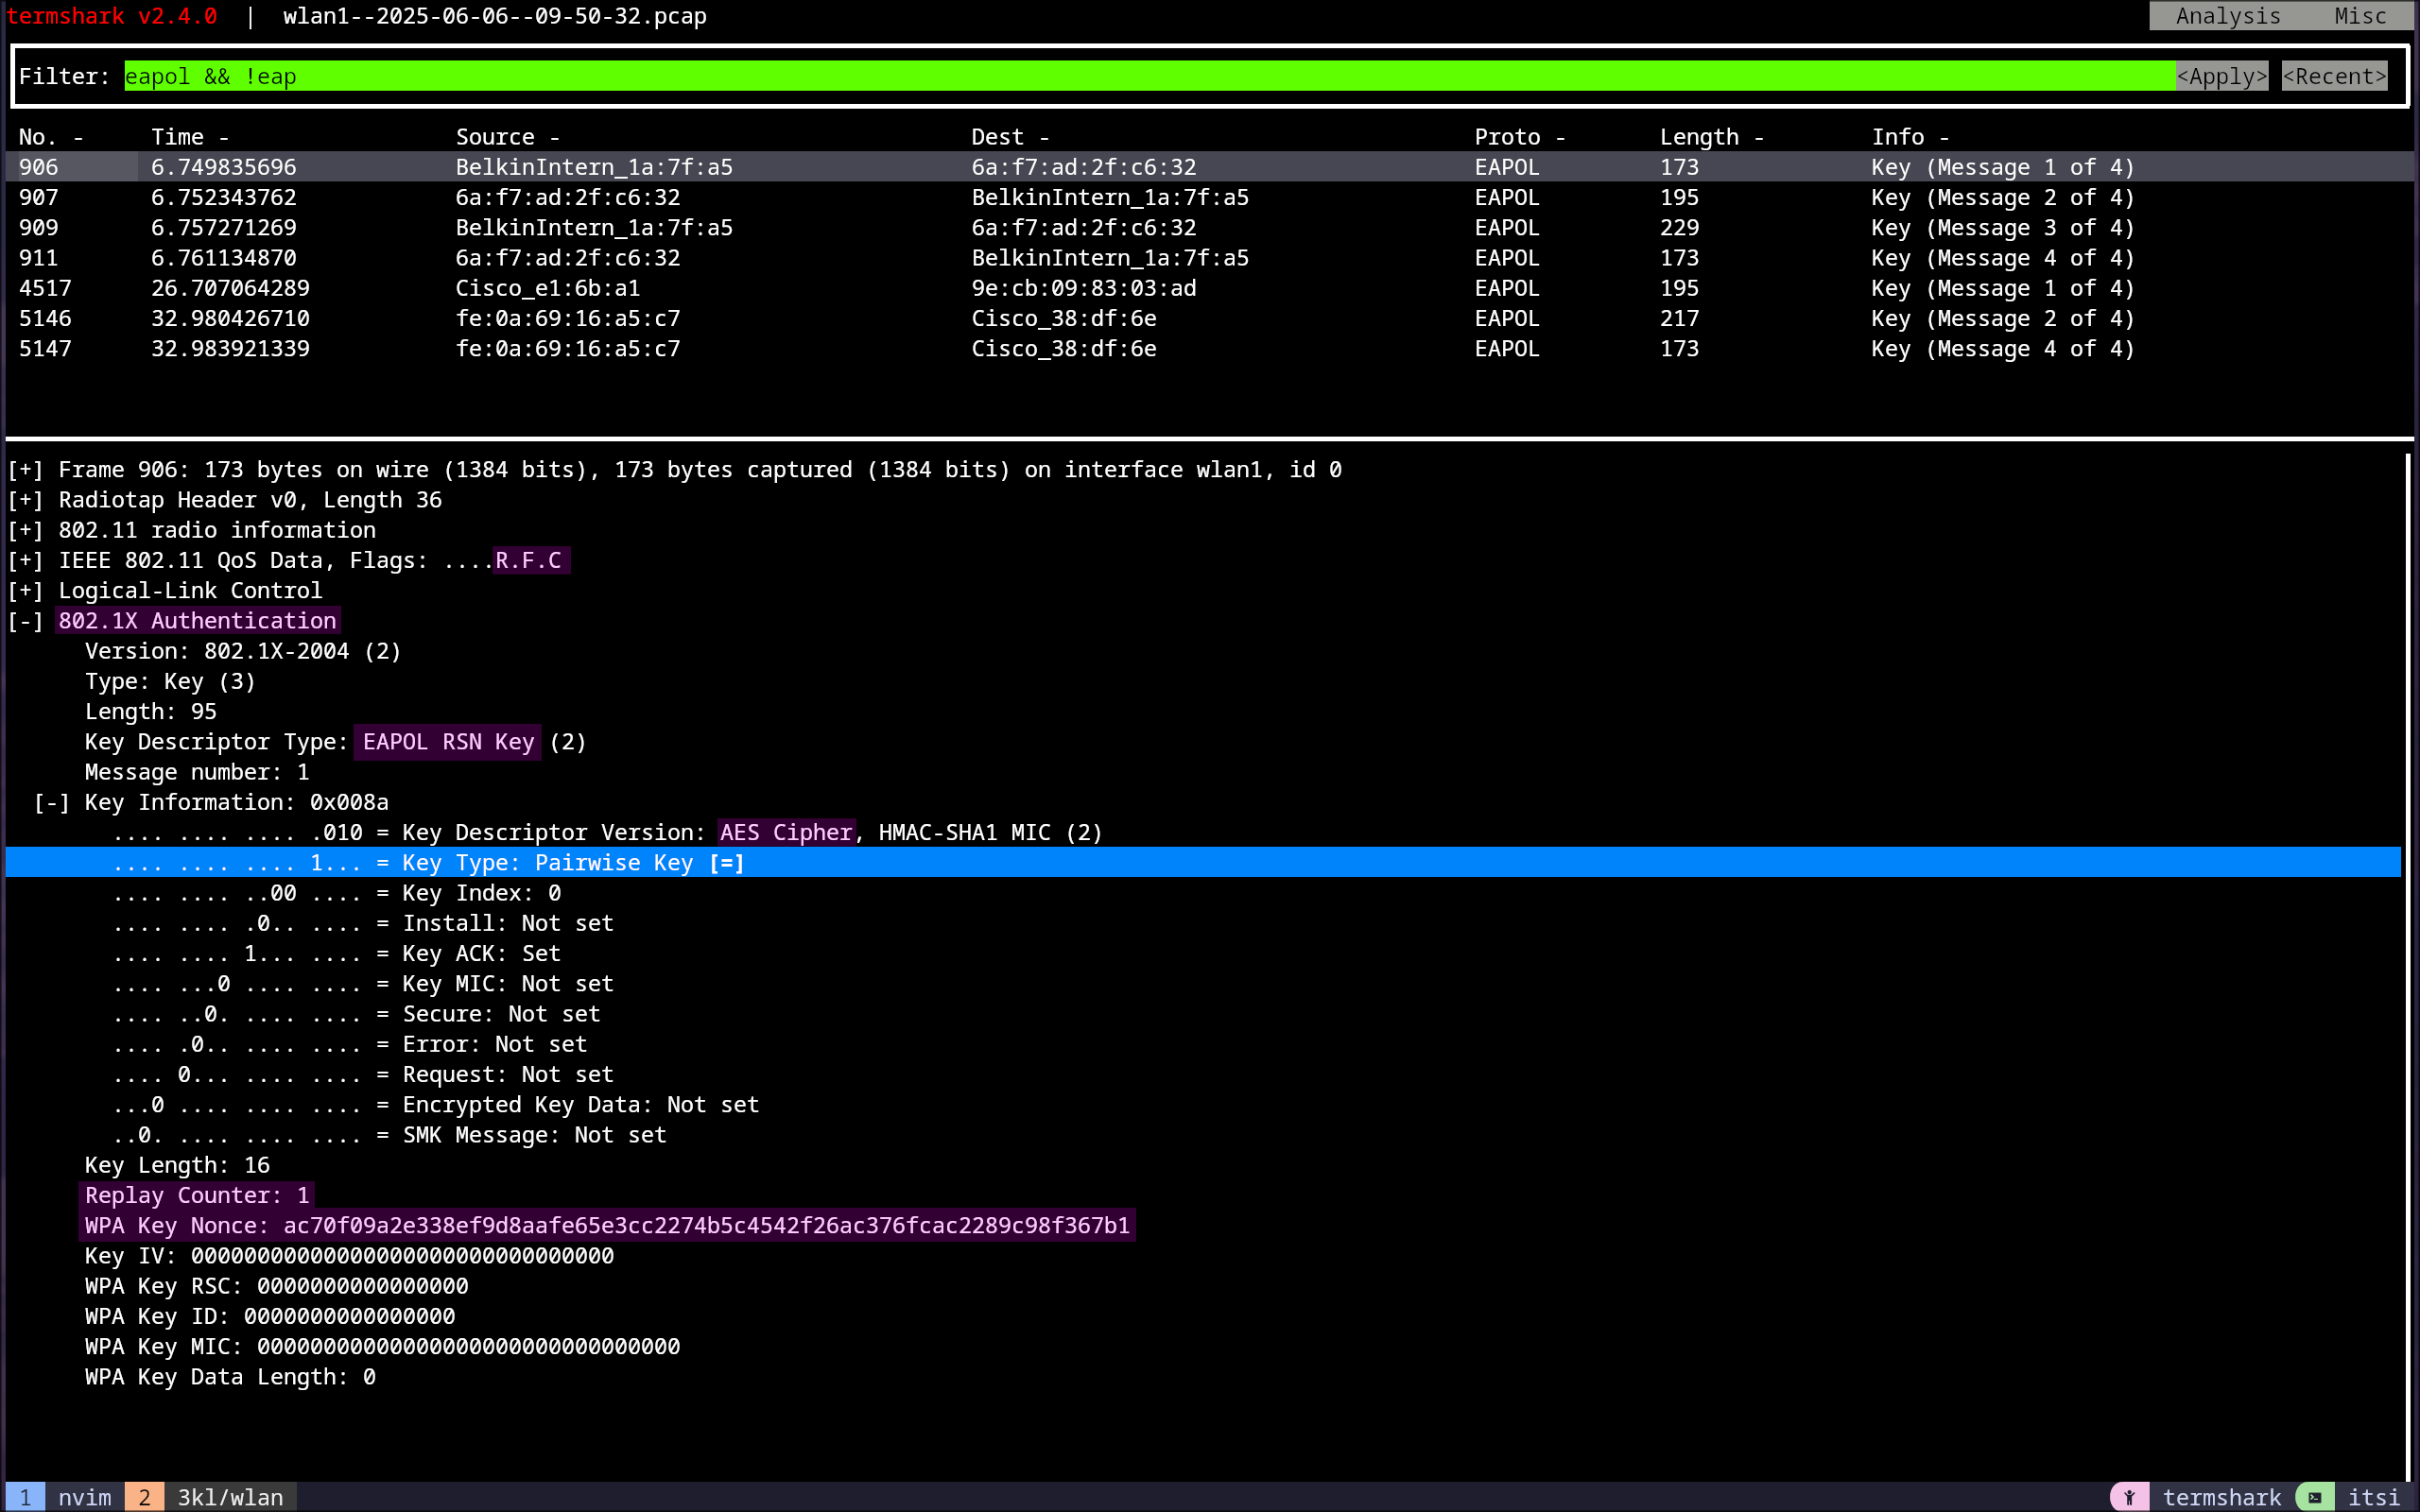
\includegraphics[scale=0.13]{images/hadnshake1.png}
    \centering
    \caption{First frame of the 4-Way Handshake}
\end{figure}
\subsubsection{4-Way Handshake Message 2}
The supplicant sends its \texttt{SNonce} with a \texttt{MIC} (which also changes the \texttt{Key Information Field} and sets the \texttt{Key MIC} flag to 1) to the authenticator. After the AP receives this, the \texttt{PTK (Pairwise Transient Key)} is verified. If the \texttt{MIC} is not valid, the \texttt{MLME-DEAUTHENTICATE.request} primitive is used to terminate the association \cite{noauthor_ieee_2016-1, admin_4-way_2019}. \nl
Figure 23 displays this frame.
\begin{figure}[!ht]
    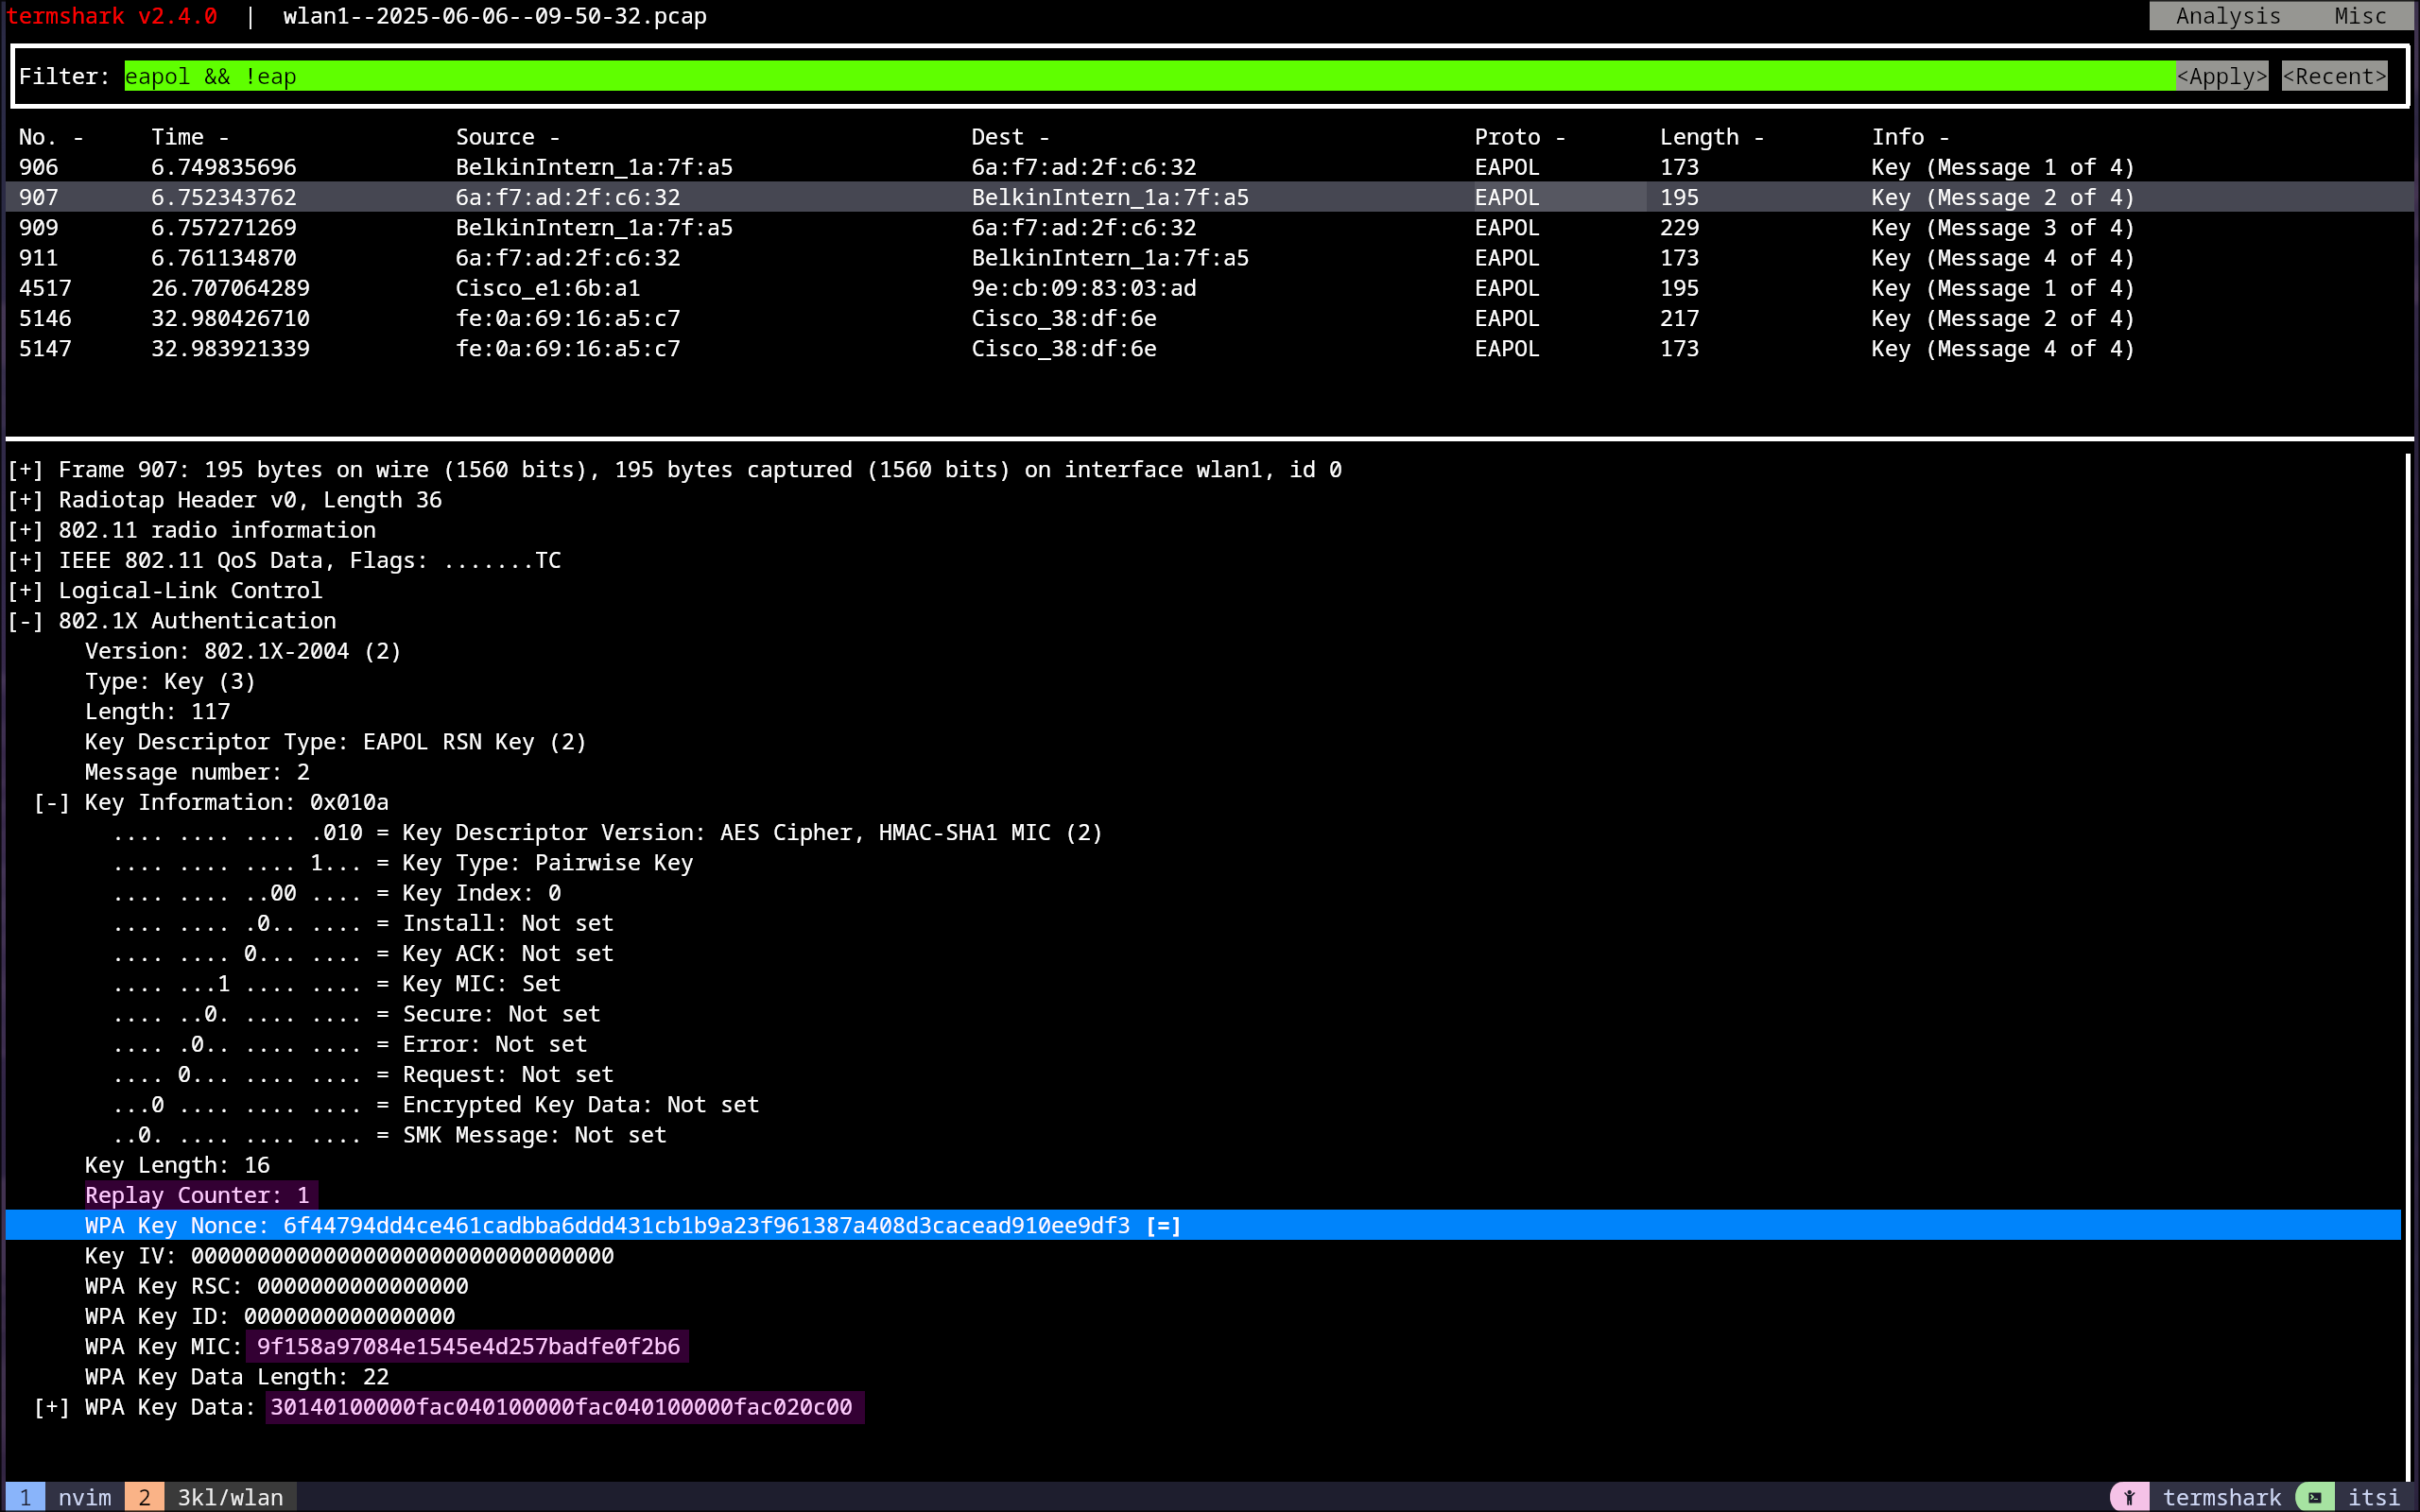
\includegraphics[scale=0.13]{images/handskahe2.png}
    \centering
    \caption{Second frame of the 4-Way Handshake}
\end{figure} \newpage
\subsubsection{4-Way Handshake Message 3}
The authenticator checks the \texttt{MIC}, and if it is valid, it generates the \texttt{GTK (Group Transient Key)}, which gets encapsulated in the \texttt{Key Data} field. The replay counter is incremented, and the install flag in the \texttt{Key Information} field is set to 1, along with the \texttt{Key ACK} and \texttt{Key MIC} fields. Upon receiving this, the supplicant verifies the \texttt{MIC} and \texttt{ANonce}, and if successful, constructs Message 4 \cite{noauthor_ieee_2016-1}. 
Figure 24 displays this frame.
\begin{figure}[!ht]
    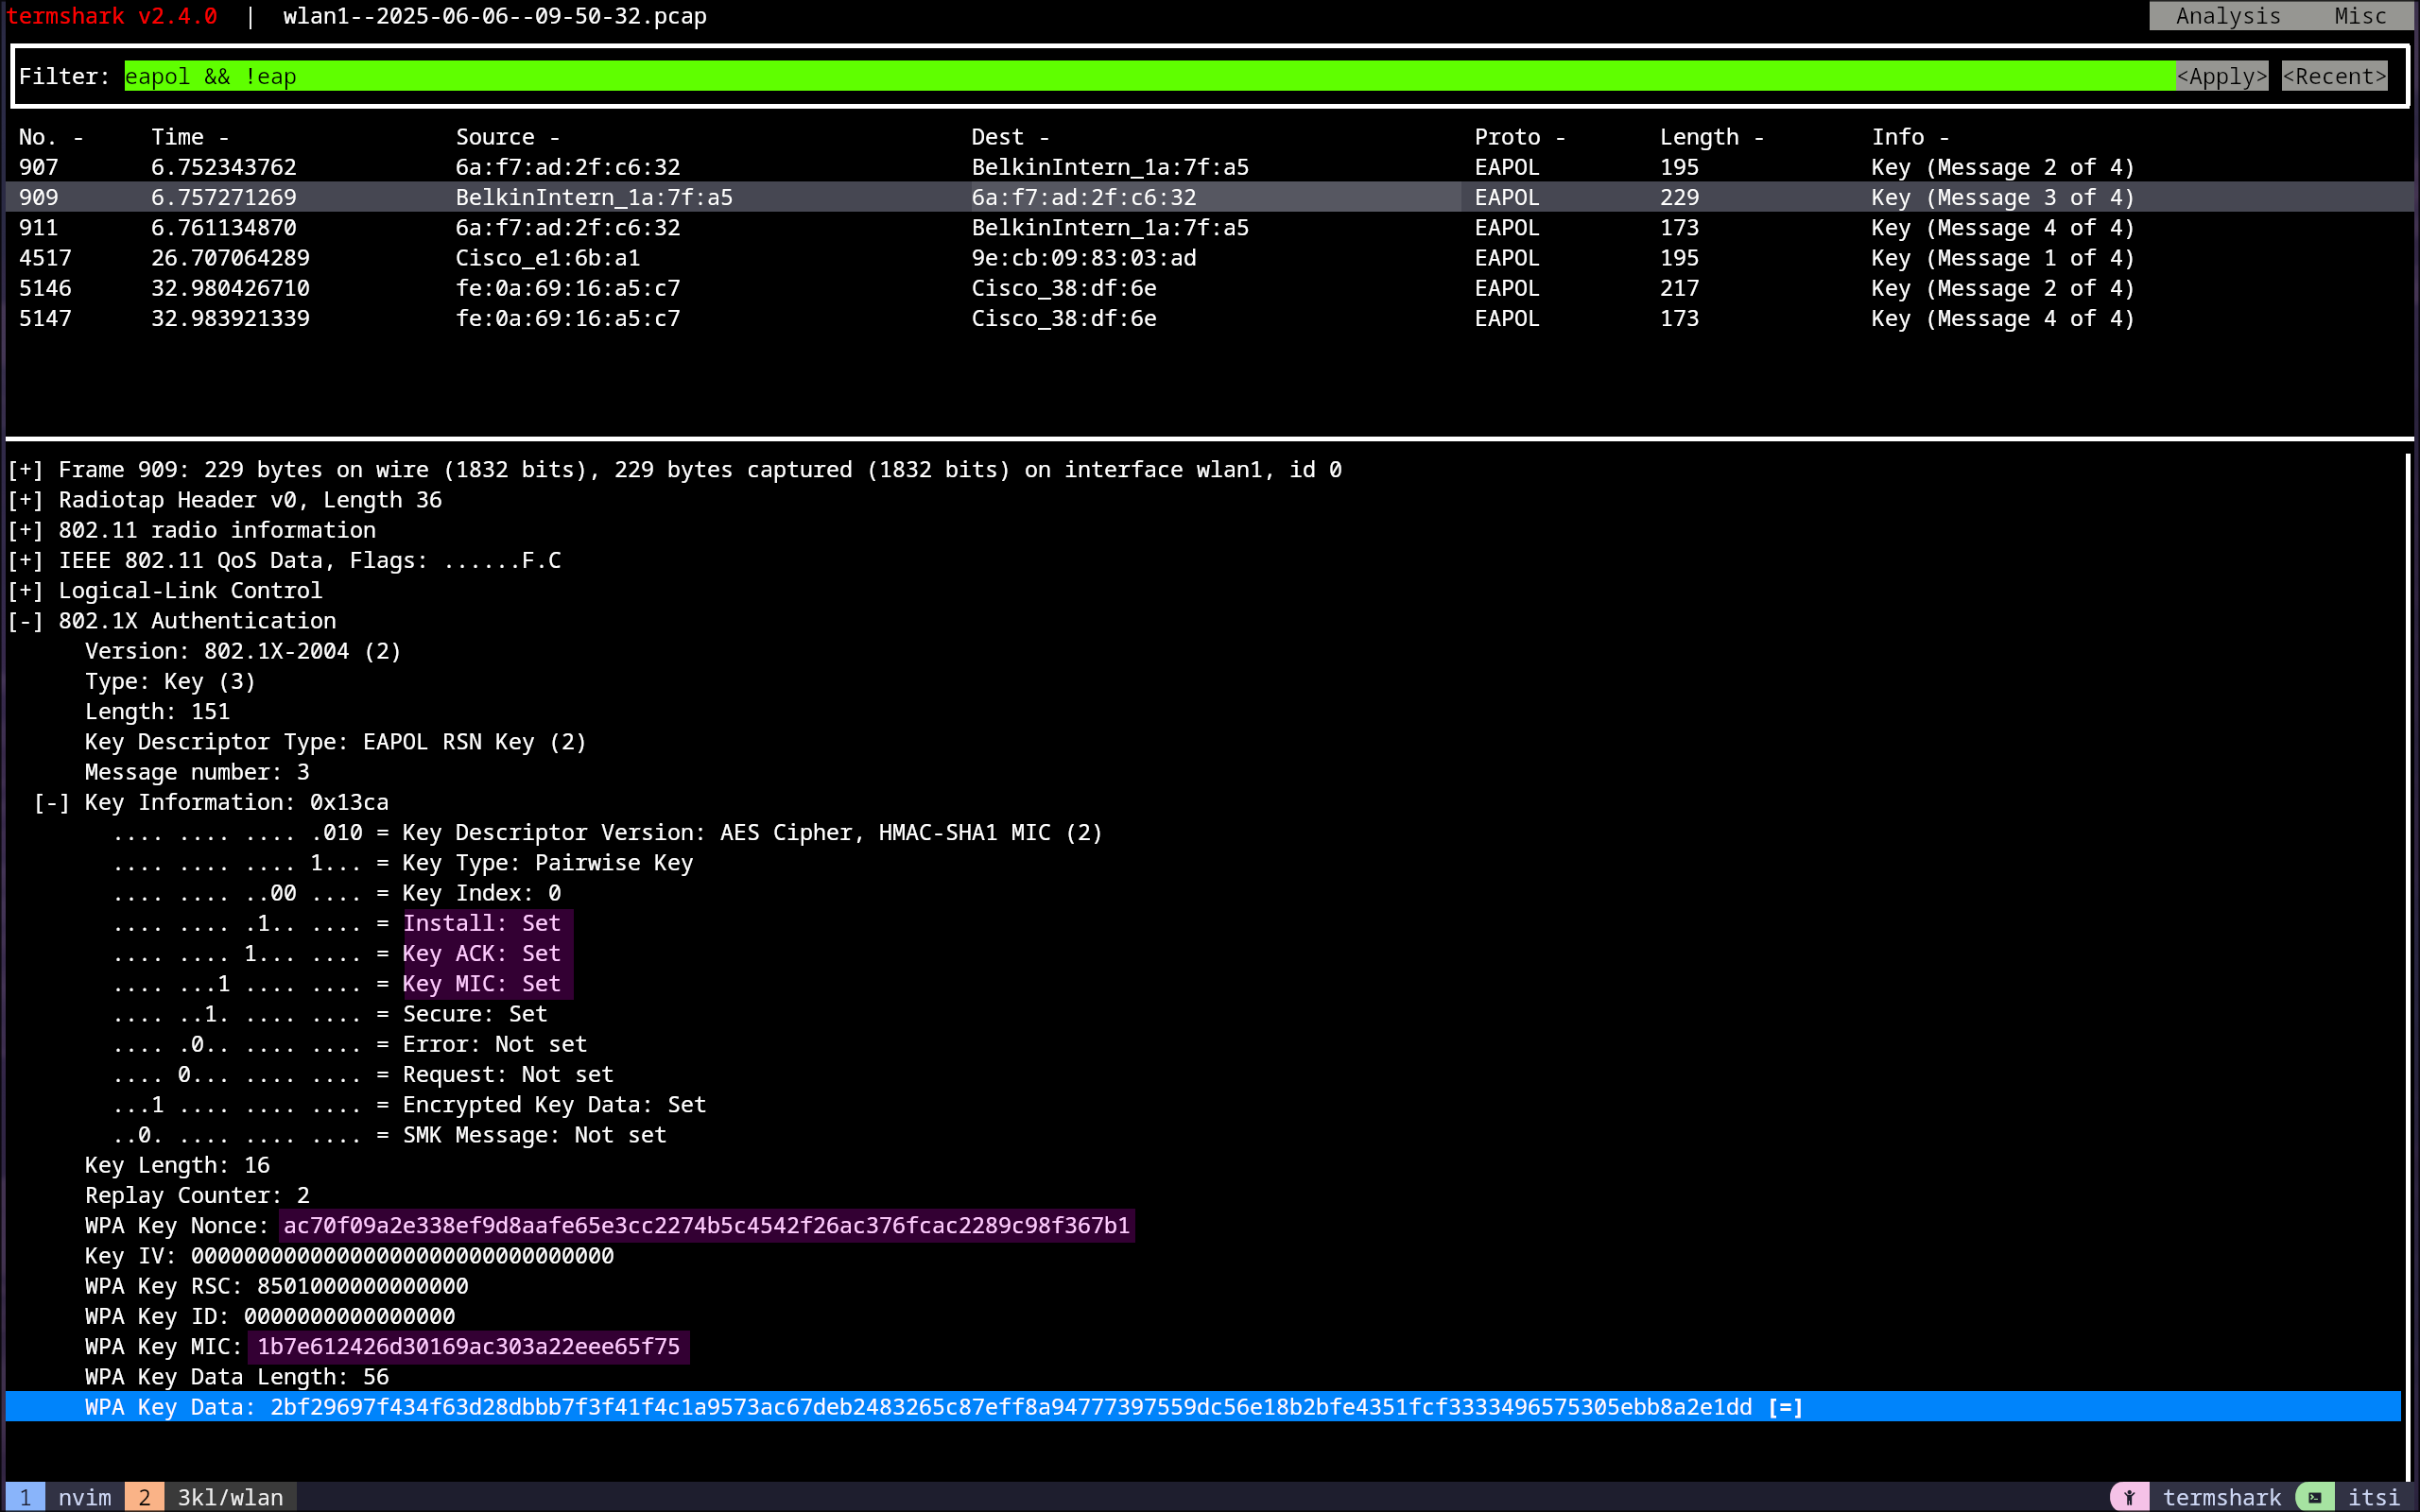
\includegraphics[scale=0.13]{images/handshake3.png}
    \centering
    \caption{Third frame of the 4-Way Handshake}
\end{figure}
\subsubsection{4-Way Handshake Message 4}
The supplicant sends a frame with the \texttt{Key ACK} field set to 0 and only a \texttt{MIC} as a final \texttt{OK}, indicating that everything needed for the communication is installed \cite{admin_4-way_2019}. \nl
Figure 25 displays the final frame of the handshake.

\begin{figure}[!ht]
    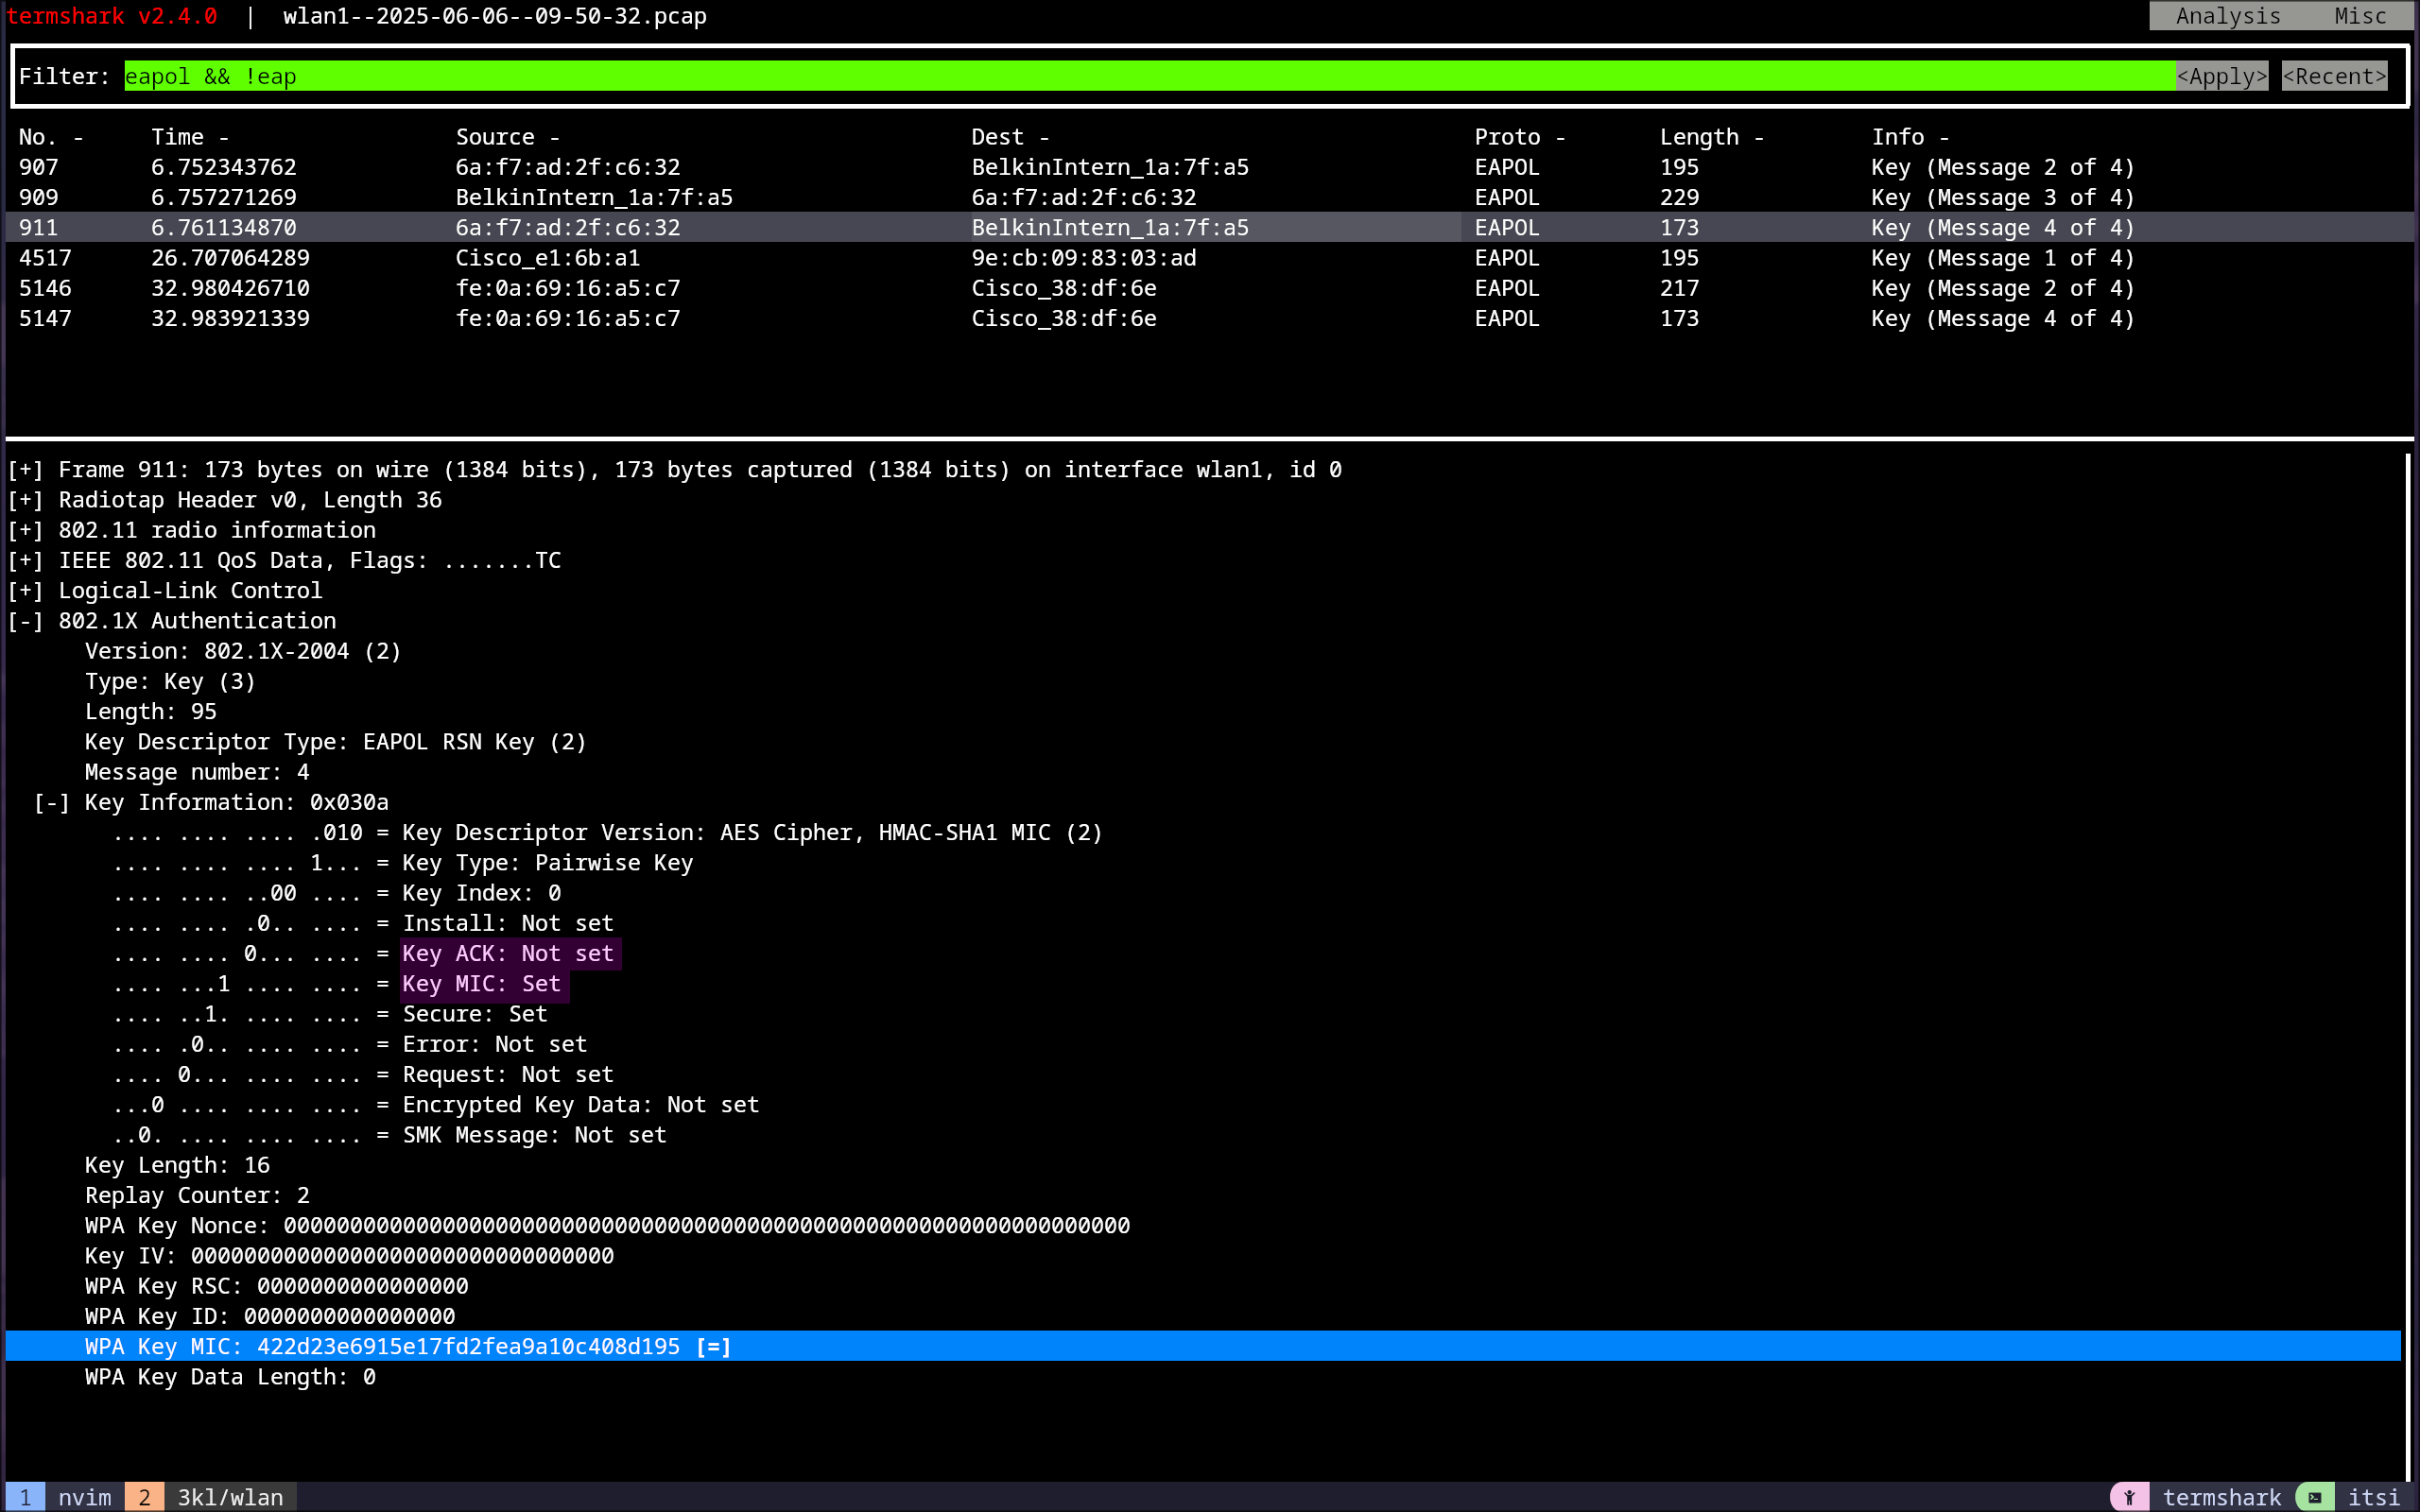
\includegraphics[scale=0.13]{images/handshake4.png}
    \centering
    \caption{Fourth frame of the 4-Way Handshake}
\end{figure} \newpage
\subsection{Cracking the Password}
To finally crack the password, the following \texttt{aircrack-ng} command was used: \nl
\texttt{aircrack-ng -w pwlist -b B4:75:0E:1A:7F:A5 thing*.cap} \nl
This command uses the \texttt{-w} option to set a wordlist, which is the top 100k used password list, to which I append the correct password, as seen in Figure 26. The \texttt{-b} option sets the \texttt{BSSID} to use, and lastly, \texttt{thing*.cap} tells \texttt{aircrack-ng} to use all \texttt{.cap} files starting with \texttt{thing} as the name. Once the command is run and the password is found, it will be displayed, which can also be seen in Figure 26 \cite{noauthor_aircrack-ng_nodate}. \nl
\begin{figure}[!ht]
    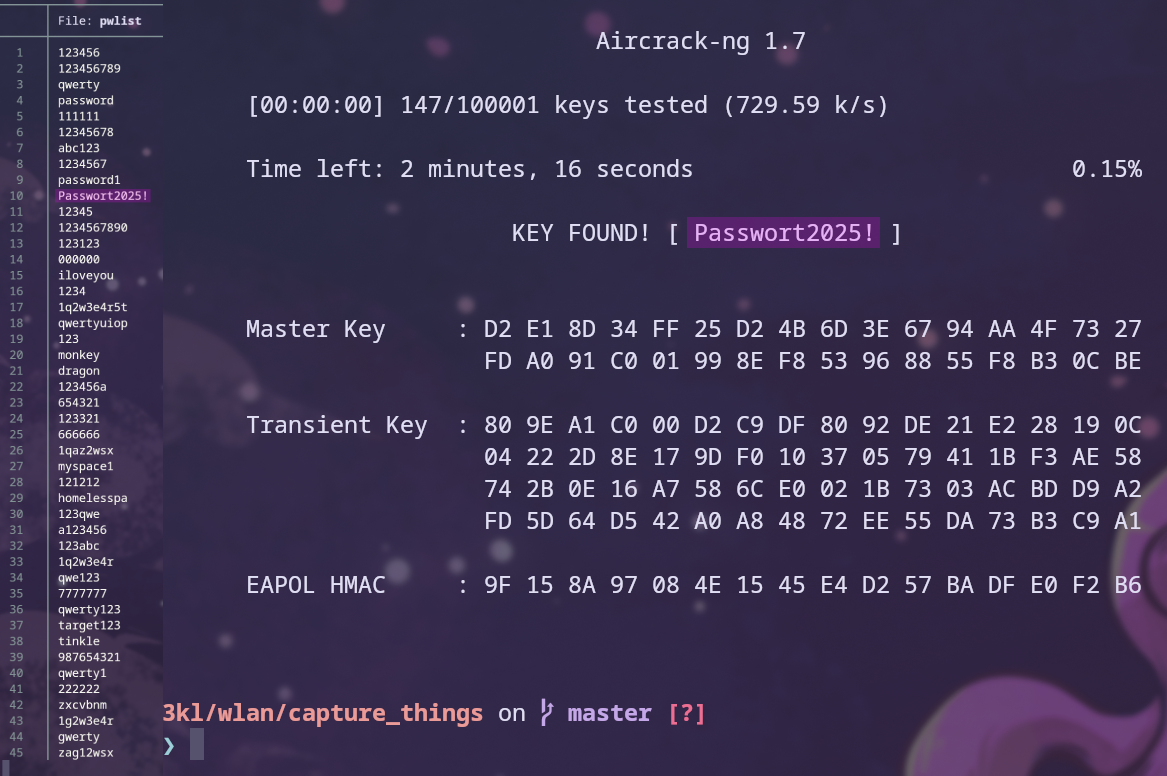
\includegraphics[scale=0.33]{images/pwlist.png}
    \centering
    \caption{Showing the cracked password}
\end{figure}
\subsubsection{Testing My Own Wi-Fi}
Now I wanted to do something extra to test my home Wi-Fi to see if it holds up. \nl
To do this, I reran the same commands as in the sections above. \nl
After obtaining the hash, I used \texttt{hcxpcapngtool -o home.22000 -E WLAN-homeF2 pcap/mehrstuff.pcapng} to convert the Wireshark capture from the background to a \texttt{.22000} file so I could use \texttt{hashcat} on my PC to crack my password without simply adding the password to the list and see how long it takes. This command uses \texttt{hcxtools} to extract the hashed password for a given \texttt{SSID} from a capture file so it can be used for hashcat. To do this, the \texttt{-o} option was used to set the output file, as well as the \texttt{-E} option to set the \texttt{SSID}, and lastly, the location of the input file to use. \nl
On my Windows PC, I used the following hashcat command: \nl
\texttt{.\textbackslash{}hashcat.exe -m 22000 .\textbackslash{}home.22000 -a 3 -w 3 ?u?u?u?u?u?u?u?u?u?u?u?u?u?u?u?u?u} \nl
This command uses the \texttt{-m} option to determine the type of hash, which in this case is a \texttt{WPA-PBKDF2-PMKID+EAPOL} hash. The \texttt{-a 3} option sets the attack mode to 3, which is a brute force mask attack, and \texttt{-w 3} sets the workload profile to be aggressive and use as many system resources as possible. Lastly, the \texttt{?u} is a placeholder for uppercase alphanumeric characters (A-Z), since my password is not in a wordlist and only consists of 17 alphanumeric uppercase characters \cite{noauthor_cracking_wpawpa2_nodate, noauthor_mask_attack_nodate}. \nl
However, as seen in Figures 27 and 28 on the next page, the length of the password caused hashcat to overflow on my system, and the Bitwarden password strength calculator indicates it would take centuries to crack. Therefore, I see this as a success for my security.\newpage 
\begin{figure}[!ht]
    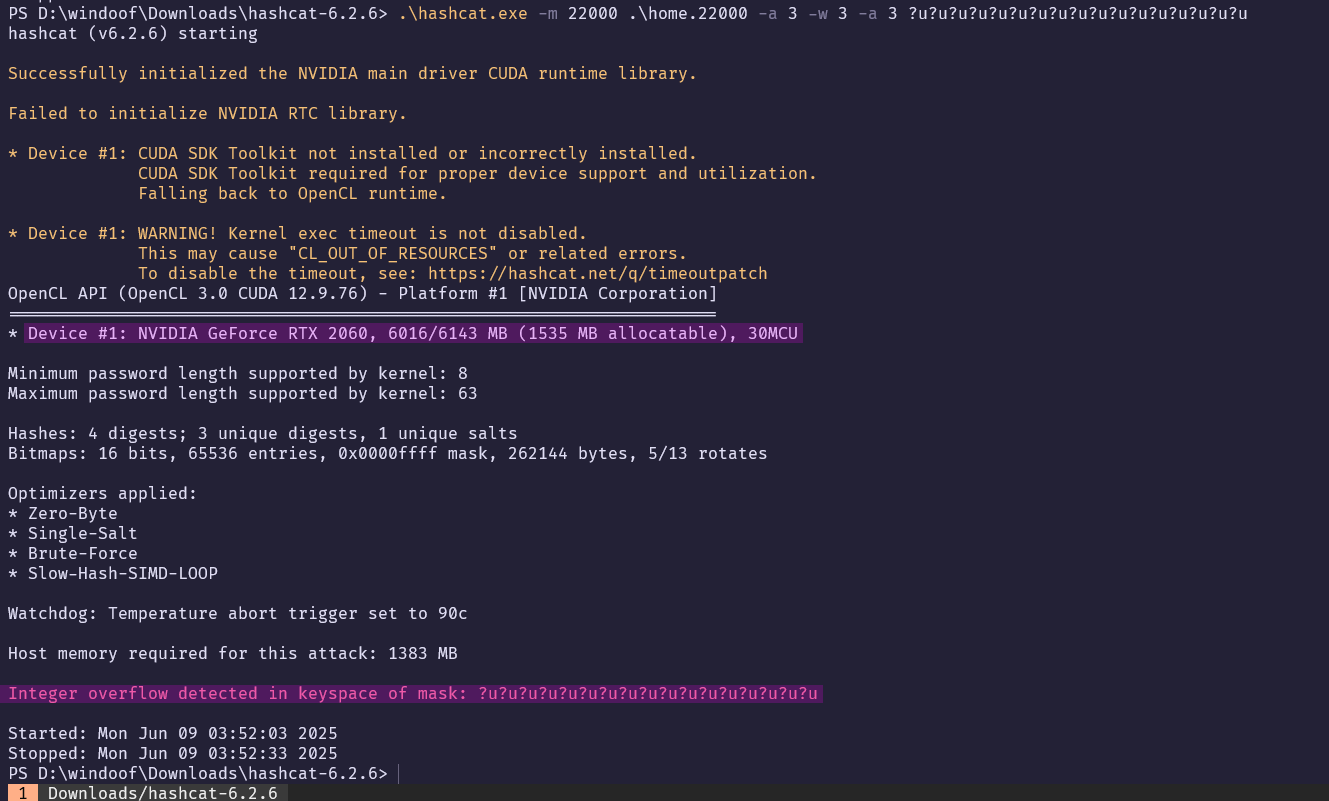
\includegraphics[scale=0.33]{images/hashcat.png}
    \centering
    \caption{Showing the output of the hashcat command}
\end{figure}
\begin{figure}[!ht]
    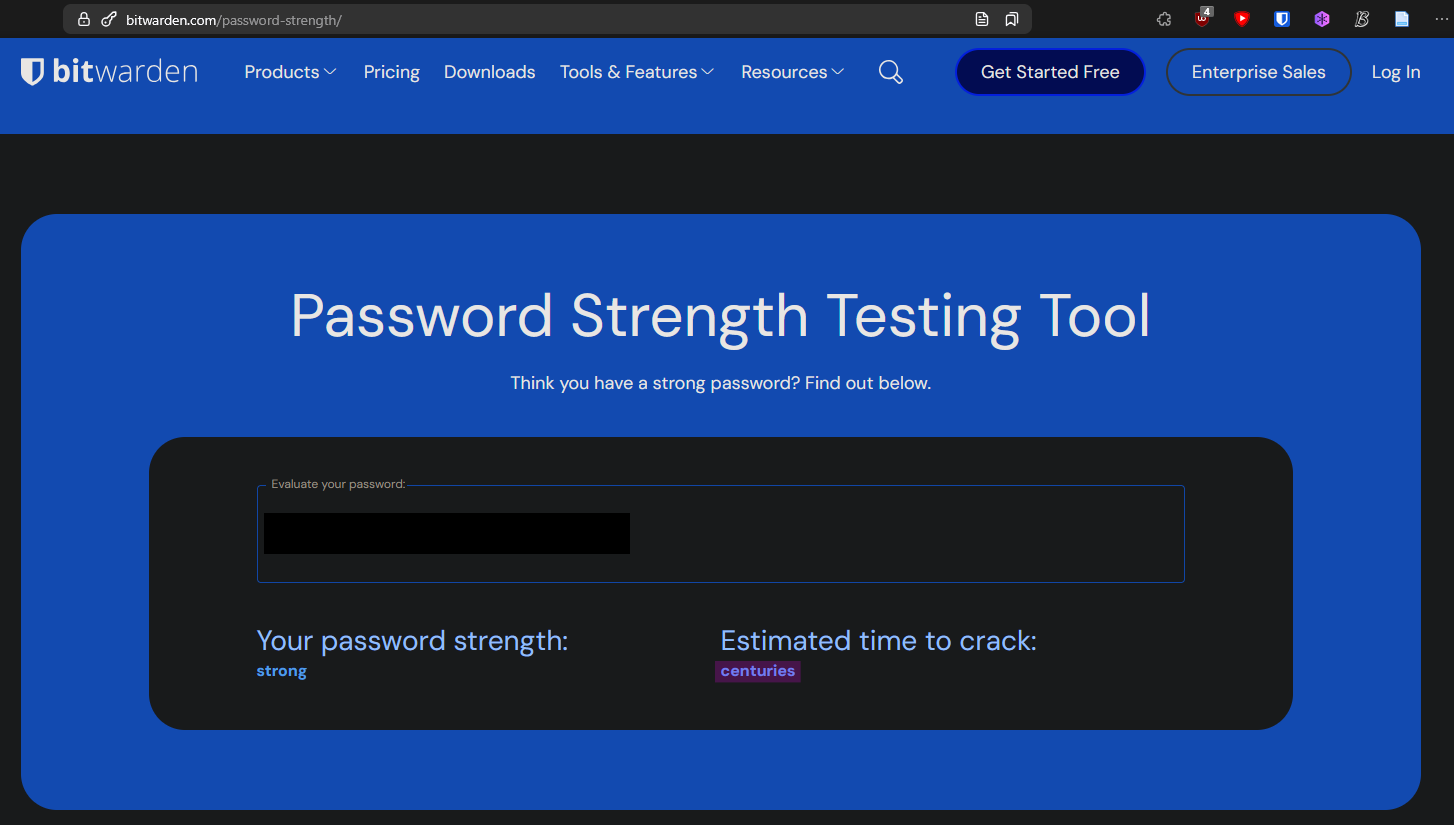
\includegraphics[scale=0.3]{images/wlanpwtest.png}
    \centering
    \caption{Showing the time estimation for my password to be cracked}
\end{figure} \newpage
\subsection{Mitigations of This Attack}
To make such attacks harder, or even impossible, or less likely to occur, there are mainly three ways to achieve this: \nl
- Using a strong password \nl
- Forcing WPA3 \nl
- Segmenting the network \nl
All of these work together, and to illustrate the point, a scenario for a home network will be used that incorporates all of them while trying to reduce the increased effort of higher security as little as possible. \nl \nl
Since most homes have IoT devices or printers that can't use newer encryption standards, the \texttt{Guest Network} feature on the router will be used, which will have all IoT devices such as printers, etc. If possible, the internet speed will be limited, and a somewhat secure password will be used. \nl
For the main network, a strong password is used, and \texttt{WPA3} is enforced. To reduce the burden of long passwords, \texttt{NFC} cards and \texttt{QR Codes} can be used to connect to the Wi-Fi in a more convenient way. \nl \nl
This achieves all of the above-mentioned points and protects the family from an outdated device, like a printer, being a backdoor to their network and potentially spying on their local traffic or, due to the weaker encryption, risking an attacker breaking into their home Wi-Fi.
\subsubsection{How WPA3 improves security}
The first upgrade of \texttt{WPA3} is the improvement of the encryption algorithm, which is now \texttt{256-bit Galois/Counter Mode Protocol (GCMP-256)}, significantly improving upon WPA2. \nl \nl
The main improvement is the Dragonfly handshake, which is resistant to dictionary attacks and provides forward secrecy. It makes use of zero-knowledge proofs, and for each authentication, a new key is generated. Due to the zero-knowledge proof, the password is never actually transmitted \cite{noauthor_wpa3_nodate}. \nl
The handshake is essentially a \texttt{SPEKE (Simple Password Exponential Key Exchange)}, which works like this: \nl
\begin{enumerate}
    \item Both Alice and Bob share a password \( P \).
    \item They use a known transformation to derive a point \( G \) on the elliptic curve \( E \).
    \item Then Alice and Bob each randomly pick a value in the domain of the prime \( p \).
    \item Alice randomly picks \( a \) and Bob randomly picks \( b \).
    \item They exchange \( aG \) and \( bG \).
    \item Then both parties compute \( K \) as usual in the Diffie-Hellman key exchange.
\end{enumerate} \nl
This makes offline dictionary attacks not feasible because an attacker can guess \( G \), but they can't find \( aG \) and \( bG \) due to the hardness of the mathematical problem. Since \( a \) and \( b \) were randomly chosen, \( K \) cannot be computed, and even if the password is guessed correctly, it is still very unlikely that the two random numbers \( a \) and \( b \) were also guessed correctly \cite{noauthor_wpa3_nodate}.
\subsubsection{Possible WPA3 Attacks}
There are mainly four types of attacks used against WPA3, which are:
\begin{enumerate}
    \item Timing-based side-channel attacks
    \item Cache-based side-channel attacks
    \item Downgrade attacks
    \item Denial of Service
\end{enumerate}
The first two attacks are \texttt{side-channel attacks}, which are any attacks based on extra information that can be gathered because of the fundamental way a computer protocol or algorithm is implemented, rather than flaws in the design of the protocol or algorithm itself. For example, in a \texttt{timing-based side-channel attack}, the computation time of an action gives the attacker more information about the system, allowing them to exploit that and gain more information, such as comparing the computation timing for two passwords. A cache-based side-channel attack would involve the attacker monitoring the accesses made by the victim in a shared physical system, like a virtualized environment, to gain information in that manner \cite{noauthor_side-channel_2025}.\nl \nl
In the context of WPA3, a \texttt{timing-based side-channel attack} involves measuring the time it takes for an access point (AP) to respond to commit frames, which may leak information about the password \cite{noauthor_dragonblood_2024}. \nl \nl
A \texttt{cache-based side-channel attack} can occur if the attacker is able to observe the memory access patterns of the victim's device when constructing the commit frame, which would reveal information about the password \cite{noauthor_dragonblood_2024}. \nl \nl
Downgrade attacks leverage the coexistence of WPA2 and WPA3 in an access point. The goal is to create a rogue access point that lures legitimate clients away from the genuine access point and forces them to use WPA2, allowing the attacker to capture the handshake and crack it offline \cite{noauthor_dragonblood_2024}. \nl \nl
Lastly, due to the increased complexity of the Dragonfly handshake, simply flooding the access point with commit frames can lead to high CPU usage and potentially slow the access point down \cite{noauthor_dragonblood_2024}. \nl \nl


\newpage
\section{References}
\bibliography{IEEEabrv,zotero}
\newpage
\section{List of figures}
\listoffigures
\newpage
\section{List of snippets}
\listoflistings
\end{document}
